\documentclass[compress,table,xcolor=table]{beamer}
\mode<presentation>
\usetheme{Montpellier}
\hypersetup{pdfstartview={Fit}}

\usecolortheme{spruce}
\useoutertheme{smoothbars}

\setbeamertemplate{bibliography item}[text]
\usepackage[utf8]{inputenc}
\usepackage{caption}
\usepackage{enumitem}
\usepackage{dirtytalk}
\usepackage{multirow}

\definecolor{light-gray}{gray}{0.95}

\usepackage{listings}
\lstset{
backgroundcolor = \color{light-gray},
basicstyle=\footnotesize\ttfamily,
language=C++,
breaklines=true,
tabsize=2,
%numbers=left,
%firstnumber=1,
escapeinside={(*@}{@*)}
}

\usepackage{url}

\setlist[itemize,1]{label=$\bullet$}
\setlist[itemize,2]{label=$\bullet$}
\setlist[itemize,3]{label=$\bullet$}

\begin{document}

\title{Qt training course}

\frame{\titlepage}

% Intro %
\section{Introduction}

\begin{frame}
  \frametitle{What is Qt?}
  \small
  \begin{columns}
    \begin{column}{0.5\textwidth}
    \begin{itemize} 
      \item Cross-platform application development framework for desktop,
        embedded, mobile and web:
        \begin{itemize}
        \item Linux,
        \item OS X,
        \item Windows,
        \item VxWorks,
        \item QNX,
        \item Android,
        \item iOS,
        \item BlackBerry,
        \item Sailfish OS,
        \item Symbian,
        \item others.
        \end{itemize}
    \end{itemize}
    \end{column}
    \begin{column}{0.5\textwidth}
      \footnotesize
      \begin{itemize}
      \item Has modular architecture.
      \item Not a programming language by its own, but uses extended C++.
      \item Available under various licenses, both commercial and free software.
      \item Implements its own build system, but it's also usable with
      third-party build tools.
      \item Comes with its own IDE -- called {\em Qt Creator}.
      \item Provides a simple unit-testing framework.
      \item More info at \url{https://wiki.qt.io/About_Qt}.
      \end{itemize} 
    \end{column}
  \end{columns}
\end{frame}

\subsection{History}
\begin{frame}
  \frametitle{Qt's history (1988 - 2000)}
  \scriptsize
  \begin{itemize}
    \item {\em 1988} -- Haavard Nord\footnote{\tiny Later the first CEO of Trolltech}
      commissioned by a Swedish company to develop a C++ GUI framework.
    \item {\em 1990} -- The first version of Qt concieved by Haavard Nord and
      Eirik Chambe-Eng\footnote{\tiny Later the first president of Trolltech} as the
      library for developing a database application for ultrasound images.
    \item {\em 1991} -- Beginning of development of the initial, proprietary version.
    \item {\em 1994} -- The {\em Quasar Technologies} company was founded, later
      renamed to {\em Troll Tech} and finally to {\em Trolltech}.
    \item {\em 1995} -- Troll Tech publicly released Qt version 0.90 for X11/Linux.
      The first commercial contract from Metis - a Norwegian company.
    \item {\em 1996} -- The European Space Agency became the second Qt customer.
    \item {\em 1997} -- Qt 1.2 and 1.3 released.
    \item {\em 1998} -- Matthias Ettrich, joins Trolltech. Qt 1.4 released.
    \item {\em 1999} -- Qt won the LinuxWorld award for best library/tool.
      Qt 2.0 released.
    \item {\em 2000} -- New Qt windowing system, Qt/Embedded released.
  \end{itemize}
\end{frame}

\begin{frame}
  \frametitle{Qt's history (2001 - 2012)}
  \scriptsize
  \begin{itemize}
    \item {\em 2001} -- Qt 3.0 with support for multiple database environments,
      multiple languages, multiple monitors and support for Mac OS X and a new
      Qt Designer GUI builder released.
    \item {\em 2005} -- Qt 4.0 with fully made-over API, released
      under commercial and GPL 2.0 licenses for all major platforms.
    \item {\em 2006} -- Trolltech IPO\footnote{\tiny Initial public offering --
      \say{stock market launch}}. 
      Qt used in millions of devices worldwide from Sharp to Motorola.
    \item {\em 2008} -- Acquisition of Trolltech by  Nokia, renamed to
      \say{Qt Software at Nokia}.
    \item {\em 2009} -- Qt Creator released. Qt version 4.5 released under LGPL v2.1.
    \item {\em 2010} -- Qt Quick launched, integration with WebKit. Qt 4.7 released
      with support for the Symbian OS.
    \item {\em 2011} -- Qt commercial licensing business acquired by
      Digia\footnote{\tiny\url{https://digia.fi/}}.
    \item {\em 2012} -- Digia acquires all rights to Qt as \say{Digia, Qt}.
      Qt 5.0 released with new modularized codebase, consolidation of QPA\footnote
      {\tiny Qt Platform Abstraction}, Qt Quick 2, and more support for mobile
      platforms.
  \end{itemize}
\end{frame}

\begin{frame}
  \frametitle{Qt's history (recent)}
  \scriptsize
  \begin{itemize}
    \item {\em 2012} -- Framework development of Qt 5 moved to open governance
      at \url{https://qt-project.org}.
    \item {\em 2013} -- Launch of the Qt pre-built software stack. Launch of
      Qt WebEngine, integrating {\em Chromium}'s web capabilities into Qt.
    \item {\em 2014} -- Digia transferred the Qt business and copyrights to their
      wholly owned subsidiary; \say{The Qt Company}.
    \item {\em 2015} -- 20\textsuperscript{th} anniversary of Qt's first
      public release.
      \say{One Qt} site unification completed -- \url{https://www.qt.io/}.
      More than 800K Qt developers worldwide.
    \item {\em 2016} -- Latest version: Qt 5.8.
  \end{itemize}
\end{frame}

\begin{frame}
  \frametitle{Modules -- Qt essentials\footnote
  {\tiny Source: \url{https://doc.qt.io/qt-5/qtmodules.html}}}

  \small
  \begin{itemize}
  \item Fundamental Qt modules, available on all supported development and
    testing platforms.
  \item Generic and useful for the majority of Qt applications.
  \end{itemize}

  \tiny
  \begin{columns}
    \begin{column}{0.48\textwidth}
      \rowcolors{2}{green!80!yellow!50}{green!70!yellow!40}
      \begin{tabular}{|p{0.28\textwidth}|p{0.65\textwidth}|}
      \hline
      \textbf{Module} & \textbf{Purpose} \\
      \hline
      {\em Qt Core} & Core non-graphical classes used by other modules. \\
      \hline
      {\em Qt GUI} & Base classes for graphical user interface (GUI) components.
        Includes OpenGL. \\
      \hline
      {\em Qt Multimedia} & Classes for audio, video, radio and camera functionality. \\
      \hline
      {\em Qt Multimedia Widgets} & Widget-based classes for implementing
        multimedia functionality. \\
      \hline
      {\em Qt Network} & Classes to make network programming easier and more portable. \\
      \hline
      {\em Qt QML} & Classes for QML and JavaScript languages. \\
      \hline
      {\em Qt Quick} & A declarative framework for building highly dynamic
        applications with custom user interfaces. \\
      \hline
      \end{tabular}
    \end{column}
    \begin{column}{0.48\textwidth}
      \rowcolors{2}{green!80!yellow!50}{green!70!yellow!40}
      \begin{tabular}{|p{0.34\textwidth}|p{0.56\textwidth}|}
      \hline
      \textbf{Module} & \textbf{Purpose} \\
      \hline
      {\em  Qt Quick Controls} & Reusable Qt Quick based UI controls to create
        classic desktop-style user interfaces. \\
      \hline
      {\em  Qt Quick Dialogs} & Types for creating and interacting with system
        dialogs from a Qt Quick application. \\
      \hline
      {\em  Qt Quick Layouts} & Layouts are items that are used to arrange
        Qt Quick 2 based items in the user interface. \\
      \hline
      {\em  Qt SQL} & Classes for database integration using SQL. \\
      \hline
      {\em  Qt Test} & Classes for unit testing Qt applications and libraries. \\
      \hline
      {\em  Qt Widgets} & Classes to extend Qt GUI with C++ widgets. \\
      \hline
      \end{tabular}
    \end{column}
  \end{columns}
\end{frame}

\begin{frame}
  \frametitle{Modules -- Qt add-ons (MP, IPC, IO, sensors)\footnote
  {\tiny Source: \url{https://doc.qt.io/qt-5/qtmodules.html}}}

  \small
  \begin{itemize}
  \item Modules bringing additional value for specific purposes.
  \item May be available only on certain platforms.
  \end{itemize}

  \tiny
  \begin{columns}
    \begin{column}{0.48\textwidth}
      \rowcolors{2}{green!80!yellow!50}{green!70!yellow!40}
      \begin{tabular}{|p{0.38\textwidth}|p{0.56\textwidth}|}
      \hline
      \textbf{Module} & \textbf{Purpose} \\
      \hline
      Qt Concurrent & Classes for writing multi-threaded programs without using low-level threading primitives. \\
      \hline
      Qt D-Bus & Classes for inter-process communication over the D-Bus protocol. \\
      \hline
      Qt Location & Displays map, navigation, and place content in a QML application. \\
      \hline
      Qt Positioning & Provides access to position, satellite and area monitoring classes.\\
      \hline
      \end{tabular}
    \end{column}
    \begin{column}{0.48\textwidth}
      \rowcolors{2}{green!80!yellow!50}{green!70!yellow!40}
      \begin{tabular}{|p{0.35\textwidth}|p{0.56\textwidth}|}
      \hline
      \textbf{Module} & \textbf{Purpose} \\
      \hline
      Qt Sensors & Provides access to sensor hardware and motion gesture recognition. \\
      \hline
      Qt Serial Port & Provides access to hardware and virtual serial ports. \\
      \hline
      Qt Bluetooth & Provides access to Bluetooth hardware. \\
      \hline
      Qt NFC & Provides access to Near-Field communication (NFC) hardware. \\
      \hline
      Qt Print Support & Classes to make printing easier and more portable.\\
      \hline
      \end{tabular}
    \end{column}
  \end{columns}
\end{frame}

\begin{frame}
  \frametitle{Modules -- Qt add-ons (platform-specific, graphics, XML)\footnote
  {\tiny Source: \url{https://doc.qt.io/qt-5/qtmodules.html}}}

  \tiny
  \begin{columns}
    \begin{column}{0.48\textwidth}
      \rowcolors{2}{green!80!yellow!50}{green!70!yellow!40}
      \begin{tabular}{|p{0.38\textwidth}|p{0.56\textwidth}|}
      \hline
      \textbf{Module} & \textbf{Purpose} \\
      \hline
      Active Qt & Classes for applications which use ActiveX and COM \\
      \hline
      Qt Windows Extras & Provides platform-specific APIs for Windows. \\
      \hline
      Qt X11 Extras & Provides platform-specific APIs for X11. \\
      \hline
      Qt Mac Extras & Provides platform-specific APIs for OS X. \\
      \hline
      Qt Android Extras & Provides platform-specific APIs for Android. \\
      \hline
      Qt Quick Extras & Provides a specialized set of controls that can be
      used to build interfaces in Qt Quick.\\
      \hline
      Qt Quick widgets & Provides a C++ widget class for displaying a Qt Quick
      user interface. \\
      \hline
      \end{tabular}
    \end{column}
    \begin{column}{0.48\textwidth}
      \rowcolors{2}{green!80!yellow!50}{green!70!yellow!40}
      \begin{tabular}{|p{0.38\textwidth}|p{0.55\textwidth}|}
      \hline
      \textbf{Module} & \textbf{Purpose} \\
      \hline
      Qt Image Formats & Plugins for additional image formats: TIFF, MNG, TGA, WBMP. \\
      \hline
      Qt Canvas 3D & Enables OpenGL-like 3D drawing calls from Qt Quick applications using JavaScript. \\
      \hline
      Qt Graphical Effects & Graphical effects for use with Qt Quick 2. \\
      \hline
      Qt Image Formats & Plugins for additional image formats: TIFF, MNG, TGA, WBMP. \\
      \hline
      Qt XML & C++ implementations of SAX and DOM.\\
      \hline
      Qt XML Patterns & Support for XPath, XQuery, XSLT and XML schema validation. \\
      \hline
      \end{tabular}
    \end{column}
  \end{columns}
\end{frame}

\begin{frame}
  \frametitle{Modules -- Qt add-ons (web)\footnote
  {\tiny Source: \url{https://doc.qt.io/qt-5/qtmodules.html}}}

  \scriptsize
      \rowcolors{2}{green!80!yellow!50}{green!70!yellow!40}
      \begin{tabular}{|p{0.27\textwidth}|p{0.65\textwidth}|}
      \hline
      \textbf{Module} & \textbf{Purpose} \\
      \hline
      Qt WebChannel & Provides access to QObject or QML objects from HTML clients
      for seamless integration of Qt applications with HTML/JavaScript clients.\\
      \hline
      Qt WebEngine & Provides a QML API to run web applications using the Chromium
      browser project.\\
      \hline
      Qt WebEngine Widgets & Provides a C++ API to run web applications using
      the Chromium browser project.\\
      \hline
      Qt WebEngine Core	& Provides a public API shared by both Qt WebEngine and
      Qt WebEngine Widgets.\\
      \hline
      Qt WebSockets & Provides WebSocket communication compliant with RFC 6455.\\
      \hline
      Qt WebView & Displays web content in a QML application by using APIs native
      to the platform, without the need to include a full web browser stack.\\
      \hline
      Qt SVG & Classes for displaying the contents of SVG files. Supports a subset
      of the SVG 1.2 Tiny standard.\\
      \hline
      \end{tabular}
\end{frame}

\begin{frame}
  \frametitle{Qt official training resources}
  \begin{itemize}
    \item {\em Website root} -- \url{https://www.qt.io/}
    \item {\em Documentation} -- \url{http://doc.qt.io/}
    \item {\em API reference} -- \url{http://doc.qt.io/qt-5.6/reference-overview.html}
    \item {\em Training and events} -- \url{https://www.qt.io/events/}
    \item {\em YouTube channel} -- \url{https://www.youtube.com/user/QtStudios/}
    \item {\em Wiki} -- \url{https://wiki.qt.io/}
  \end{itemize}
\end{frame}

\subsection{This training course}

\begin{frame}
  \frametitle{Accompanying source files}
  \begin{itemize}
  \item \texttt{examples/} -- complete suite of working Qt projects
    \begin{itemize}
    \item \textbf{\texttt{01\_trivial/}} -- Trivial examples like
	    \say{hello world} on the
	    console, with minimal GUI and with XML-defined GUI, and
	    examples showing the use of Qt's basic utility classes.
    \item \textbf{\texttt{02\_basic/}} -- Examples showing the fundamental
	    basics of GUI programming in Qt, like the signal/slot mechanism,
	    basic widgets, layouts, etc.
    \item \textbf{\texttt{03\_qml/}} -- Examples showing the QML and Qt Quick
	    programming basics.
    \item \textbf{\texttt{build\_all.sh}} -- Shell script building the examples
	    in a separate directory tree in directory \texttt{\_build}.

    \end{itemize}
  \end{itemize}
\end{frame}



% Qt development %
\section{Getting started}
% Build process %
\subsection{Qt's build process and tools}
\begin{frame}
  \frametitle{Qt's build process and tools}
  \begin{itemize}
    \item The process of building Qt applications is fairly complex.
    \item Qt provides tools which greatly simplify the build process.
    \item Command line tools:
      \begin{itemize}
        \item \texttt{qmake} -- build script generator,
        \item \texttt{moc} -- metaobject compiler,
        \item \texttt{rcc} -- resource compiler, 
        \item \texttt{uic} -- user interface compiler.
      \end{itemize}
    \item Qt Creator -- cross-platform Qt-specific IDE / RAD tool.
  \end{itemize}
\end{frame}

\begin{frame}
  \frametitle{\texttt{qmake} -- build script generator}
  \begin{itemize}
    \item \texttt{qmake} is a platform-independent generator of platform-specific
      build scripts, similar to \texttt{cmake}\footnote{\url{https://cmake.org/}}.
      \begin{itemize}
        \item Unix Makefiles,
        \item NMake Makefiles,
        \item MS Visual Studio project files,
        \item XCode,
        \item etc.
      \end{itemize}
    \item The generated build scripts invoke the compiler and the other
      command-line tools (\texttt{moc}, \texttt{rcc}, \texttt{uic}, etc.)
      in a platform-specific way.
    \item The project files used by \texttt{qmake} are however,
      platform-independent.
  \end{itemize}
\end{frame}

\begin{frame}[fragile]
  \frametitle{{\texttt .pro} -- \texttt{qmake} project files}
  \small
  \begin{itemize}
    \item The project files are structured text files containing all information
      required by \texttt{qmake} to build an application, library, or plugin.
    \item The source files and other resources are usually specified declaratively
      by assigning values to predefined variables:
      \begin{itemize}
        \item \begin{verbatim}
VARIABLE  = list "of values"
\end{verbatim}
        \item \begin{verbatim}
VARIABLE += additional values
\end{verbatim}
        \item \begin{verbatim}
VARIABLE -= values "to be" \
            removed
\end{verbatim}
      \end{itemize}
    \item Values containing white-spaces must be enclosed in double quotes.
    \item Value initialization can span multiple lines if the newline is escaped.
    \item Variables can be dereferenced by prepending \verb@$$@ before the
      identifier:
      \begin{itemize}
      \item \verb@MY_VAR = $$VARIABLE@
      \end{itemize}
    \item Comments start with a hash sign \verb@#@
      \begin{itemize}
      \item \verb@# This comment spans to the end of the line@
      \end{itemize}
  \end{itemize}
\end{frame}

\begin{frame}
  \frametitle{{\texttt .pro} -- common variables}
  \begin{center}
  \rowcolors{2}{green!80!yellow!50}{green!70!yellow!40}
  \begin{tabular}{|p{0.2\textwidth}|p{0.7\textwidth}|}
    \hline
    \textbf{Variable} & \textbf{Purpose} \\
    \hline
    \texttt{CONFIG} & General project configuration options \\
    \hline
    \texttt{FORMS} & A list of UI files to be processed by uic. \\
    \hline
    \texttt{HEADERS} & A list of filenames of header files used when building the project. \\
    \hline
    \texttt{QT} & Qt-specific configuration options. \\
    \hline
    \texttt{RESOURCES} & A list of resource files to be included in the final project. \\
    \hline
    \texttt{SOURCES} & A list of source code files to be used when building the project. \\
    \hline
    \texttt{TEMPLATE} & The template to use for the project. This determines whether the output of the build process will be an application, a library, or a plugin. \\
    \hline
  \end{tabular}
  \end{center}
\end{frame}

\begin{frame}
  \frametitle{{\texttt .pro} -- additional variables}
  \begin{center}
  \rowcolors{2}{green!80!yellow!50}{green!70!yellow!40}
  \begin{tabular}{|p{0.2\textwidth}|p{0.7\textwidth}|}
    \hline
    \textbf{Variable} & \textbf{Purpose} \\
    \hline
    \texttt{DESTDIR} & The directory in which the executable or binary file will be placed. \\
    \hline
    \texttt{SUBDIRS} & List of subdirectories containing sub-projects. Used
    with the \texttt{subdir} \texttt{TEMPLATE}.\\
    \hline
    \texttt{LIBS} & List of paths to link library files or a list of Unix-style
      link \texttt{-llibname} or \texttt{-Llibdir} options. \\
    \hline
    \texttt{INCLUDEPATH} & List of paths containing third-party include files. \\
    \hline
    \texttt{DEFINES} & List of preprocessor symbols which should be defined. \\
    \hline
    \texttt{PKGCONFIG} & List names of third-party packages registered with
    the \texttt{pkg-config} utility\footnote
    {\tiny\url{http://www.freedesktop.org/wiki/Software/pkg-config}}. \\
    \hline
  \end{tabular}
  \end{center}
\end{frame}

\begin{frame}
\frametitle{{\texttt .pro} -- values for \texttt{CONFIG} -- build types}
  \begin{center}
  \rowcolors{2}{green!80!yellow!50}{green!70!yellow!40}
  \begin{tabular}{|p{0.2\textwidth}|p{0.7\textwidth}|}
    \hline
    \textbf{Value} & \textbf{Meaning} \\
    \hline
    \texttt{qt\footnote{defined by default}} & The target is a Qt application
    or library and requires the Qt library and header files.\\
    \hline
    \texttt{x11} & The target is a X11 application or library.\\
    \hline
    \texttt{console} & The target is a console application. \\
    \hline
    \texttt{windows} & The target is a Windows application. \\
    \hline
    \texttt{testcase} & The target is an automated test. Only relevant when
    generating makefiles. \\
    \hline
  \end{tabular}
  \end{center}
\end{frame}

\begin{frame}
\frametitle{{\texttt .pro} -- values for \texttt{CONFIG} -- library-related}
  \begin{center}
  \rowcolors{2}{green!80!yellow!50}{green!70!yellow!40}
  \begin{tabular}{|p{0.22\textwidth}|p{0.68\textwidth}|}
    \hline
    \textbf{Value} & \textbf{Meaning} \\
    \hline
    \texttt{shared} & The target is a shared library.\\
    \texttt{dll} & \\
    \hline
    \texttt{static} & The target is a static library.\\
    \texttt{staticlib} & \\
    \hline
    \texttt{plugin} & The target is a plug-in\footnote{implies \texttt{shared}}.\\
    \hline
    \texttt{designer} & The target is a plug-in for {\em Qt Designer}.\\
    \hline
  \end{tabular}
  \end{center}
\end{frame}

\begin{frame}
\frametitle{{\texttt .pro} -- values for \texttt{CONFIG} -- build configurations}
  \begin{center}
  \rowcolors{2}{green!80!yellow!50}{green!70!yellow!40}
  \begin{tabular}{|p{0.3\textwidth}|p{0.6\textwidth}|}
    \hline
    \textbf{Value} & \textbf{Meaning} \\
    \hline
    \texttt{release} & The project is built in the release mode. \\
    \hline
    \texttt{debug} & The project is built in the debug mode. If both
    \texttt{release} and \texttt{debug} are specified, then the last one takes
    effect.\\
    \hline
    \texttt{debug\_and\_release} & The project is built in the both the release 
    and the debug mode.
    If the (default) \texttt{debug\_and\_release\_target} option is specified,
    then the debug and release files are built into separate subdirectories.
    \\
    \hline
    \texttt{build\_all} & If \texttt{debug\_and\_release} is specified,
    the project is built in both debug and release modes by default.  \\
    \hline
  \end{tabular}
  \end{center}
\end{frame}

\begin{frame}
\frametitle{{\texttt .pro} -- values for \texttt{CONFIG} -- C++ features}
  \begin{center}
  \rowcolors{2}{green!80!yellow!50}{green!70!yellow!40}
  \begin{tabular}{|p{0.25\textwidth}|p{0.65\textwidth}|}
    \hline
    \textbf{Value} & \textbf{Meaning} \\
    \hline
    \texttt{exceptions} & Exceptions should be enabled\footnote{are enabled
    by default}.  Otherwise the compiler's default behavior is used.\\
    \hline
    \texttt{exceptions\_off} & Exceptions should be disabled.
    Otherwise the compiler's default behavior is used.\\
    \hline
    \texttt{thread} & Support for threads should be enabled.
    This option is implied when \texttt{CONFIG} also includes \texttt{qt}\footnote
    {which is set by default}.\\
    \hline
    \texttt{c++11} & Support for the C++11 standard is explicitly enabled, if
    the compiler allows it. \\
    \hline
    \texttt{c++14} & Support for the C++14 standard is explicitly enabled, if
    the compiler allows it. \\
    \hline
  \end{tabular}
  \end{center}
\end{frame}

\begin{frame}
\frametitle{{\texttt .pro} -- values for \texttt{CONFIG} -- other}
  \begin{center}
  \rowcolors{2}{green!80!yellow!50}{green!70!yellow!40}
  \begin{tabular}{|p{0.20\textwidth}|p{0.70\textwidth}|}
    \hline
    \textbf{Value} & \textbf{Meaning} \\
    \hline
    \texttt{ordered} & If the \texttt{subdirs} project template is used,
    then the subdirectories listed in the \texttt{SUBDIRS} variable are
    built in the same order in which they are listed. \\
    \hline
    \texttt{warn\_on} & The compiler should output as many warnings as possible. \\
    \hline
    \texttt{warn\_off} & The compiler should output as few warnings as possible.
    If both \texttt{warn\_on} and \texttt{warn\_off} values are specified, then
    the last one takes effect.\\
    \hline
    \texttt{rtti} & RTTI should be enabled. Otherwise the compiler's default
    behavior is used.\\
    \hline
    \texttt{rtti\_off} & RTTI should be disabled. Otherwise the compiler's default
    behavior is used.\\
    \hline
  \end{tabular}
  \end{center}
\end{frame}

\begin{frame}
  \frametitle{{\texttt .pro} -- project templates}
  \begin{center}
  \rowcolors{2}{green!80!yellow!50}{green!70!yellow!40}
  \begin{tabular}{|p{0.2\textwidth}|p{0.7\textwidth}|}
    \hline
    \textbf{\texttt{TEMPLATE =}} & \textbf{Generated output} \\
    \hline
    \texttt{app}\footnote{the default} & Makefile building an application executable \\
    \hline
    \texttt{lib} & Makefile building a link library \\
    \hline
    \texttt{subdirs} & Makefile containing rules for building sub-projects \\
    \hline
    \texttt{aux\footnote{only in Qt 5}} & Makefile for builds where the compiler
      does not need to be invoked. \\
    \hline
    \texttt{vcapp} & MSVC project for building an application executable \\
    \hline
    \texttt{vclib} & MSVC project for building a link library \\
    \hline
    \texttt{vcsubdirs} & MSVC solution containing several sub-projects \\
    \hline
  \end{tabular}
  \end{center}
\end{frame}

\begin{frame}[fragile]
  \frametitle{{\texttt .pro} -- \texttt{qmake} built-ins and flow control}
  \small
  \begin{itemize}
    \item Support for simple programming constructs allow to describe different
      build processes for different platforms and environments:
      \begin{itemize}
      \item Contents of other \texttt{.pro} files can be included:
\begin{verbatim}
include(another.pro)
\end{verbatim}
      \item Conditional structures:
\begin{verbatim}
<condition> {
    <conditionally-executed-commands>
}
\end{verbatim} for example:
\begin{verbatim}
win32 { SOURCES += win32_utils.cpp }
\end{verbatim}
      \item For-each loops:
\begin{verbatim}
LIST = list of values
for(ITEM, LIST) {
    MY_VAR = $$ITEM
}
\end{verbatim}
      \end{itemize}
  \end{itemize}
\end{frame}

\begin{frame}[fragile]
  \frametitle{Building on the command line with \texttt{qmake}}
  \begin{columns}
    \begin{column}[t]{0.47\textwidth}
      Building in the source tree:
      \begin{verbatim}
$> cd ${PROJECT_ROOT}
$> qmake project_name.pro
$> make
      \end{verbatim}
      Cleanup in the source tree:
      \begin{verbatim}
$> make distclean
      \end{verbatim}
    \end{column}
    \begin{column}[t]{0.53\textwidth}
      Building in a separate directory tree:
      \begin{verbatim}
$> cd ${PROJECT_ROOT}
$> mkdir _build_dir
$> cd _build_dir
$> qmake ../project_name.pro
$> make
      \end{verbatim}
      Cleanup in a separate directory tree:
      \begin{verbatim}
$> rm -rf _build_dir
      \end{verbatim}
    \end{column}
  \end{columns}
\end{frame}

\begin{frame}
  \frametitle{\texttt{moc}\footnote
    {\url{http://doc.qt.io/qt-5.6/moc.html}} -- metaobject compiler}
  \begin{itemize}
    \item \texttt{moc} -- abbreviation for {\em metaobject compiler},
      is an external metaprogramming tool which implements Qt's extensions to
      C++
      \begin{itemize}
        \item the signal and slot mechanism,
        \item dynamic properties,
        \item special type-casts,
        \item extended type-info and reflection.
      \end{itemize}
    \item During a build it pre-processes the C++ source files and generates
      new temporary, intermediate C++ files, which are compiled into the final
      executable.
    \item Triggered for example by the \texttt{Q\_OBJECT}, \texttt{Q\_PROPERTY},
      \texttt{Q\_CLASSINFO} and several other macros in the C++ source code.
  \end{itemize}
\end{frame}

\begin{frame}
  \frametitle{\texttt{rcc}\footnote
    {\url{http://doc.qt.io/qt-5.6/rcc.html}} -- resource compiler}
  \begin{itemize}
    \item \texttt{rcc} or {\em resource compiler}, is an external tool which
      compiles and embeds external resource files into the built executable.
    \item It allows to distribute the executable together with frequently
      used resources and data bundled into a single file.
    \item Common resource types:
      \begin{itemize}
        \item bitmaps,
        \item icons,
        \item sounds,
        \item scripts or programs in other languages (GLSL),
        \item translations,
        \item etc.
      \end{itemize}
    \item The resource files are specified in \texttt{.rc} or \texttt{.qrc} format.
  \end{itemize}
\end{frame}

\begin{frame}[fragile]
  \frametitle{Qt resource system\footnote
    {\url{http://doc.qt.io/qt-5.6/resources.html}} -- \texttt{.qrc} file}
  \small
  \begin{itemize}
    \item XML-based format
    \item Specifies the external files which should be compiled into the
      executable or into an external resource file.
    \item Example
    \begin{lstlisting}
	<!DOCTYPE RCC>
	<RCC version="1.0">
	  <qresource>
    	    <file>icons/copy.png</file>
    	    <file>icons/cut.png</file>
    	    <file>icons/new.png</file>
    	    <file>icons/open.png</file>
    	    <file>icons/paste.png</file>
    	    <file>icons/save.png</file>
	  </qresource>
	</RCC>
    \end{lstlisting}
  \end{itemize}
\end{frame}

\begin{frame}[fragile]
  \frametitle{Qt resource system -- \texttt{.qrc} file (cont.)}
  \begin{itemize}
    \footnotesize
    \item Resources compiled into the executable can be accessed from the same
      executable by using special paths or \texttt{QUrl}s\footnote
       {\url{http://doc.qt.io/qt-5.6/qurl.html}}:
      \begin{itemize}
        \item \verb@:/path/to/dir/filename.ext@
        \item \verb@qrc:///path/to/dir/filename.ext@
      \end{itemize}
    \item The embedded resource filename can be changed with the \verb@alias@
      attribute:
      \begin{itemize}
        \item Declaration:
        \begin{lstlisting}[basicstyle=\scriptsize\ttfamily]
	<file alias="icon-cut.png">icons/cut.png</file>
        \end{lstlisting}
        \item Accessed as: \verb@:/icon-cut.png@
      \end{itemize}
    \item The path to the resource can be changed with the \verb@prefix@
      attribute:
      \begin{itemize}
        \item Declaration:
        \begin{lstlisting}[basicstyle=\scriptsize\ttfamily]
	<qresource prefix="/res/img">
	  <file alias="icon-cut.png">icons/cut.png</file>
	</qresource>
        \end{lstlisting}
        \item Accessed as: \verb@:/res/img/icon-cut.png@
      \end{itemize}
  \end{itemize}
\end{frame}

\begin{frame}
  \frametitle{\texttt{uic}\footnote
    {\url{doc.qt.io/qt-5.6/uic.html}} -- user interface compiler}
  \begin{itemize}
    \item \texttt{uic} or {\em user interface compiler}, reads the user interface
      definition files (\texttt{.ui}) and generates corresponding C++ source files.
    \item The \texttt{.ui} files are specified in the XML language and can be
      either generated by a GUI designer, for example the one integrated into
      Qt Creator, or written manually.

  \end{itemize}
\end{frame}



\subsection{Qt Creator}

\begin{frame}
  \frametitle{Qt Creator\footnote
    {\url{https://www.qt.io/ide/}} \footnote{\url{http://doc.qt.io/qtcreator/}}}
  \small
  \begin{itemize}
    \item Cross-platform IDE / rapid development tool for Qt-based applications.
    \begin{itemize}
      \item Code editor with code-completion and syntax highlighting.
      \item Project and resource management
      \item Build system integration (\texttt{qmake}, \texttt{moc}, \texttt{rcc},
        \texttt{uic}, etc.)
      \item Debugger
      \item Visual form designer for both widget-based and \texttt{qml}-based
        applications.
      \item Tool for easy internationalization and translation of texts to
        other languages.
      \item Integration with popular version control systems like git, mercurial,
        subversion and others.
      \item Configurable keyboard shortcuts.
    \end{itemize}
  \end{itemize}
\end{frame}

\begin{frame}
  \frametitle{Qt Creator -- code editor}
    \begin{figure}[!t]
    \centering
    \includegraphics[width=\textwidth]{images/qt_creator1.png}
    \end{figure}
\end{frame}

\begin{frame}
  \frametitle{Qt Creator -- form designer}
    \begin{figure}[!t]
    \centering
    \includegraphics[width=\textwidth]{images/qt_creator2.png}
    \end{figure}
\end{frame}

\begin{frame}
  \frametitle{Qt Creator -- default shortcuts for common actions\footnote
     {\url{http://doc.qt.io/qtcreator/creator-keyboard-shortcuts.html}}}
     \tiny
     \begin{columns}
       \begin{column}{0.5\textwidth}
       \rowcolors{2}{green!80!yellow!50}{green!70!yellow!40}
       \begin{tabular}{|p{0.65\textwidth}|p{0.25\textwidth}|}
         \hline
         \textbf{Action} & \textbf{Shortcut} \\
         Activate locator & Ctrl+K \\
         \hline
         Switch to Welcome mode & Ctrl+1 \\
         \hline
         Switch to Edit mode & Ctrl+2 \\
         \hline
         Switch to Design mode & Ctrl+3 \\
         \hline
         Switch to Debug mode & Ctrl+4 \\
         \hline
         Switch to Projects mode &Ctrl+5 \\
         \hline
         Switch to Analyze mode & Ctrl+6 \\
         \hline
         Switch to Help mode & Ctrl+7 \\
         \hline
         Toggle the sidebar & Alt+0 \\
         \hline
         Toggle Issues pane & Alt+1 \\
         \hline
         Toggle Search Results pane & Alt+2 \\
         \hline
         Toggle Application Output pane & Alt+3 \\
         \hline
         Toggle Compile Output pane & Alt+4 \\
         \hline
         Toggle other output panes & Alt+number \\
         \hline
         Activate Bookmarks pane & Alt+M \\
         \hline
         Activate File System pane & Alt+Y \\
         \hline
         Activate Open Documents pane & Alt+O \\
         \hline
         Activate Projects pane & Alt+X \\
         \hline
         Full screen & Ctrl+Shift+F11 \\
         \hline
       \end{tabular}
       \end{column}
       \begin{column}{0.5\textwidth}
       \rowcolors{2}{green!80!yellow!50}{green!70!yellow!40}
       \begin{tabular}{|p{0.65\textwidth}|p{0.25\textwidth}|}
         \hline
         \textbf{Action} & \textbf{Shortcut} \\
         \hline
         Open file or project & Ctrl+O \\
         \hline
         New file or project & Ctrl+N \\
         \hline
         Select all & Ctrl+A \\
         \hline
         Delete & Del \\
         \hline
         Cut & Ctrl+X \\
         \hline
         Cut line & Shift+Del \\
         \hline
         Copy & Ctrl+C \\
         \hline
         Copy line & Ctrl+Ins \\
         \hline
         Paste & Ctrl+V \\
         \hline
         Undo & Ctrl+Z \\
         \hline
         Redo & Ctrl+Y \\
         \hline
         Print & Ctrl+P \\
         \hline
         Save & Ctrl+S \\
         \hline
         Save all & Ctrl+Shift+S \\
         \hline
         Quit & Ctrl+Q \\
         \hline
         Close window & Ctrl+W \\
         \hline
         Close all & Ctrl+Shift+W \\
         \hline
         Close current file & Ctrl+F4 \\
         \hline
         Trigger a completion in this scope & Ctrl+Space \\
         \hline
       \end{tabular}
       \end{column}
     \end{columns}
\end{frame}



% Examples %
\section{Hello Qt}
\subsection{Trivial examples}

\begin{frame}
  \frametitle{Trivial examples}
  \begin{itemize}
  \item Located in the \texttt{examples/01\_trivial/} directory.
  \item Contains trivial examples, introducing the following concepts.
    \begin{itemize}
    \item Project files
    \item Console application basics
    \item GUI application basics
    \item Some of the Qt's utility classes
    \item Building projects with \texttt{qmake}.
    \end{itemize}
  \end{itemize}
\end{frame}

\subsection{Hello world - console}

\begin{frame}[fragile]
  \frametitle{Hello world -- console}
  Located in \texttt{examples/01\_trivial/01\_hello\_console/}:
  \begin{itemize}
  \item \texttt{main.cpp} -- the main and only source file
  \begin{lstlisting}[basicstyle=\scriptsize\ttfamily]
	#include <QTextStream>
 	 
	int main(void)
	{
	    QTextStream(stdout) << "Hello, console!" << endl;
	    return 0;
	}
  \end{lstlisting}
  \item \texttt{hello.pro} -- the Qt project file
  \begin{lstlisting}
	SOURCES += main.cpp
	TARGET   = hello_console
  \end{lstlisting}
  \end{itemize}
\end{frame}

\subsection{Hello world - GUI}

\begin{frame}[fragile]
  \frametitle{Hello world -- GUI}
  Located in \texttt{examples/01\_trivial/02\_hello\_gui/}:
  \begin{itemize}
  \item \texttt{main.cpp} -- the main source file
  \begin{lstlisting}[basicstyle=\scriptsize\ttfamily]
	#include <QtGui>
	#include <QApplication>
	#include <QLabel>

	int main(int argc, char* argv[])
	{
	    QApplication app(argc, argv);
	    QLabel label("<I>Hello</I>, <B>GUI</B> world!");
	    label.show();
	    return app.exec();
	}\end{lstlisting}
  \item \texttt{hello.pro} -- the project file
  \begin{lstlisting}
	(*@\alert{QT      += widgets}@*)
	SOURCES += main.cpp
	TARGET   = hello_gui
  \end{lstlisting}
  \end{itemize}
\end{frame}

\subsection{Hello world - XML-UI}

\begin{frame}
  \frametitle{Hello world -- XML-UI}
  Located in \texttt{examples/01\_trivial/03\_hello\_xml\_ui/}:

  \begin{itemize}
  \item \texttt{mainwindow.ui} -- an external XML file defining the form layout.
  \item \texttt{mainwindow.h} -- C++ header declaring the \texttt{MainWindow} class.
  \item \texttt{mainwindow.cpp} -- C++ file implementing the \texttt{MainWindow} class.
  \item \texttt{main.cpp} -- C++ file implementing the \texttt{main} function.
  \item \texttt{hello.pro} -- The Qt project file.
  \end{itemize}
\end{frame}

\begin{frame}[fragile]
  \frametitle{Hello world -- XML-UI}
  File \texttt{mainwindow.ui}

\begin{lstlisting}[basicstyle=\tiny\ttfamily,language=XML]
<?xml version="1.0" encoding="UTF-8"?>
<ui version="4.0">
 <class>MainWindow</class>
 <widget class="QMainWindow" name="MainWindow">
  <property name="geometry">
   <rect>
    <x>0</x><y>0</y><width>200</width><height>100</height>
   </rect>
  </property>
  <property name="windowTitle"><string>Hello</string></property>
  <widget class="QWidget" name="centralWidget">
   <widget class="QLabel" name="label">
    <property name="geometry">
     <rect>
      <x>40</x><y>40</y><width>120</width><height>20</height>
     </rect>
    </property>
    <property name="text">
     <string>&lt;I&gt;Hello&lt;/I&gt;, &lt;B&gt;GUI&lt;/B&gt; World!</string>
    </property>
    <property name="alignment"><set>Qt::AlignCenter</set></property>
   </widget>
  </widget>
 </widget>
</ui>
\end{lstlisting}
\end{frame}

\begin{frame}[fragile]
  File \texttt{mainwindow.h}

  \begin{lstlisting}[basicstyle=\scriptsize\ttfamily]
	#ifndef MAINWINDOW_H
	#define MAINWINDOW_H

	#include <QMainWindow>

	namespace Ui { class MainWindow; }

	class MainWindow
 	 : public QMainWindow
	{
	    Q_OBJECT
	public:
	    explicit MainWindow(QWidget *parent = 0);
	    ~MainWindow();
	private:
	    Ui::MainWindow *ui;
	};

	#endif // MAINWINDOW_H
  \end{lstlisting}
\end{frame}


\begin{frame}[fragile]
  File \texttt{mainwindow.cpp}

  \begin{lstlisting}
	#include "mainwindow.h"
	#include "ui_mainwindow.h"

	MainWindow::MainWindow(QWidget *parent)
 	 : QMainWindow(parent)
 	 , ui(new Ui::MainWindow)
	{
	    ui->setupUi(this);
	}

	MainWindow::~MainWindow()
	{
	    delete ui;
	}
  \end{lstlisting}
\end{frame}


\begin{frame}[fragile]
  File \texttt{main.cpp}

  \begin{lstlisting}
	#include "mainwindow.h"
	#include <QApplication>

	int main(int argc, char *argv[])
	{
	    QApplication a(argc, argv);
	    MainWindow w;
	    w.show();

	    return a.exec();
	}
  \end{lstlisting}
\end{frame}


\begin{frame}[fragile]
  File \texttt{hello.pro}

  \begin{lstlisting}
	TEMPLATE  = app
	QT       += core gui widgets
	TARGET    = hello_xml_ui

	SOURCES  += main.cpp mainwindow.cpp
	HEADERS  += mainwindow.h
	FORMS    += mainwindow.ui
  \end{lstlisting}

  \begin{itemize}
  \item Output:
    \begin{figure}[!t]
    \includegraphics[width=0.3\textwidth]{images/hello_gui.png}
    \end{figure}
  \end{itemize}

\end{frame}


\begin{frame}[fragile]
  \frametitle{Hello world -- QML}
  Located in \texttt{examples/01\_trivial/04\_hello\_qml/}:

  File \texttt{hello.qml}

  \begin{lstlisting}[basicstyle=\tiny\ttfamily]
	import QtQuick 2.0
	import QtQuick.Window 2.0

	Window {
	    width: 320; height: 130
	    color: "lightgreen"

	    Text {
	        text: "Hello QML world!"
	        y: 40
	        anchors.horizontalCenter: parent.horizontalCenter
	        font.pointSize: 24
	        font.bold: true
	    }
	    Text {
	        text: "Click to close"
	        y: 80
	        anchors.horizontalCenter: parent.horizontalCenter
	        font.pointSize: 12

	        MouseArea {
	            anchors.fill: parent
	            onClicked: Qt.quit()
	        }
	    }
}
  \end{lstlisting}

\end{frame}

\begin{frame}[fragile]
  \frametitle{Hello world -- QML}

  \begin{itemize}
  \item Running the example:
  \begin{itemize}
    \item \verb@$> qmlscene hello.qml@
  \end{itemize}
  \item Output:
    \begin{figure}[!t]
    \includegraphics[width=0.4\textwidth]{images/hello_qml.png}
    \end{figure}
  \end{itemize}
\end{frame}



% Fundamentals
\section{Core}
\subsection{Utility classes}

\begin{frame}[fragile]
  \frametitle{Core utility classes}
  \begin{itemize}
  \item Qt implements a core library of utility classes extensively used
    throughout the rest of the API.
  \begin{columns}
    \footnotesize
    \begin{column}{0.28\textwidth}
    \begin{itemize}
      \item \texttt{QString}
      \item \texttt{QByteArray}
      \item \texttt{QStringList}
      \item \texttt{QVector}
      \item \texttt{QList}
      \item \texttt{QLinkedList}
    \end{itemize}
    \end{column}
    \begin{column}{0.31\textheight}
    \begin{itemize}
      \item \texttt{QSet}
      \item \texttt{QMap}
      \item \texttt{QHash}
      \item \texttt{QVariant}
      \item \texttt{QDateTime}
      \item \texttt{QDir}
    \end{itemize}
    \end{column}
    \begin{column}{0.31\textheight}
    \begin{itemize}
      \item \texttt{QFileInfo}
      \item \texttt{QQFile}
      \item \texttt{QTextStream}
      \item \texttt{QDataStream}
      \item \texttt{QSerialPort}
      \item \ldots
    \end{itemize}
    \end{column}
  \end{columns}

  \item Project file \verb@QT += core@
  \end{itemize}
\end{frame}

\begin{frame}[fragile]
  \frametitle{\texttt{QString}\footnote
    {\url{http://doc.qt.io/qt-5.6/qstring.html}}}
  \begin{itemize}
    \item Class for storing, transferring and manipulating text in the form of
      zero-terminated character strings.
    \item Internally stores the strings in 16-bit wide \texttt{QChar}s using
      the UTF-16\footnote{\url{https://en.wikipedia.org/wiki/UTF-16}} encoding.
    \begin{itemize}
      \item Note that glyphs with Unicode code-points above $2^{16}$ are
        represented by multi-\texttt{QChar} sequences!
    \end{itemize}
    \item May use copy-on-write to reduce memory usage and to avoid the needless
      copying of data.
    \item Header \verb@#include<QString>@
  \end{itemize}
\end{frame}

\begin{frame}[fragile]
  \frametitle{\texttt{QString} -- initialization}
  \begin{itemize}
    \item Can be initialized from UTF-8\footnote
     {\url{https://en.wikipedia.org/wiki/UTF-8}}-encoded c-string literals or
     \texttt{char} arrays.
    \begin{itemize}
      \item
      \begin{verbatim}
	QString str = "hello!";
      \end{verbatim}
      \item internally calls \verb@QString::fromUtf8@.
    \end{itemize}
    \item \texttt{QStringLiteral} -- a potentially more efficient variant of
      the above. Can do the conversion to the internal implementation at
      compile-time.
    \begin{itemize}
      \item
      \begin{verbatim}
	QString str = QStringLiteral("hello!");
      \end{verbatim}
      \item only if the compiler supports it.
    \end{itemize}
    \item Also can be initialized from arrays of \texttt{QChar}s.
    \begin{itemize}
      \item
      \begin{verbatim}
	const QChar strdata[N] = {0x0055, ...};
	QString str(strdata, N);
      \end{verbatim}
    \end{itemize}
  \end{itemize}
\end{frame}

\begin{frame}[fragile]
  \frametitle{\texttt{QString} -- null vs. empty}
  \small
  \begin{itemize}
    \item Qt distinguishes between {\em null} and {\em empty} strings.
    \begin{itemize}
      \item {\em null}-string -- default-initialized or initialized from a
      \texttt{nullptr}.
      \item {\em empty}-string -- initialized from a string containing only
      the terminating zero character.
      \item {\em nonempty}-string -- any other string.
    \end{itemize}
    \item
    \begin{lstlisting}
	QString null;
	QString empty("");
	QString nonempty("abc");

	assert(null.isNull()     == true);
	assert(empty.isNull()    == false);
	assert(nonempty.isNull() == false);

	assert(null.isEmpty()    == true);
	assert(empty.isEmpty()   == true);
	assert(nonempty.isEmpty()== false);
      \end{lstlisting}
  \end{itemize}
\end{frame}

\begin{frame}[fragile]
  \frametitle{\texttt{QByteArray}\footnote
    {\url{http://doc.qt.io/qt-5.6/qbytearray.html}}}
  \begin{itemize}
    \item Class for storing, transferring and manipulating raw byte sequences,
      including text encoded in UTF-8 and other 8-bit character encodings.
    \item Can be more efficient to store texts in some character sets\footnote
    {like basic Latin} if memory resources are constrained.
    \begin{itemize}
      \item Otherwise \texttt{QString} is the preferred and recommended way to
      store text.
    \end{itemize}
    \item The data can embed zero characters.
    \item If initialized from a char array, terminating zero is preserved.

    \item Header \verb@#include<QByteArray>@
  \end{itemize}
\end{frame}

\begin{frame}[fragile]
  \frametitle{\texttt{QByteArray} -- initialization}
  \begin{itemize}
    \item Can be initialized from
    \begin{itemize}
      \item a c-string literal:
      \begin{verbatim}
	QByteArray ba("some text");
      \end{verbatim}
      \item a raw memory block:
      \begin{verbatim}
	const char raw[N] = {0x00, ...};
	QByteArray ba = QByteArray::fromRawData(raw,N);
      \end{verbatim}
      \item a \verb@std::string@:
      \begin{verbatim}
	std::string str(...);
	QByteArray ba = QByteArray::fromStdString(str);
      \end{verbatim}
      \item \ldots
    \end{itemize}
  \end{itemize}
\end{frame}

\begin{frame}[fragile]
  \frametitle{\texttt{QString}, \texttt{QByteArray} -- manipulation}
  \footnotesize
  \begin{itemize}
    \item \verb@data@ -- returns a pointer to the stored data.
    \item \verb@size@, \verb@length@ -- returns the size (in bytes) of the
    stored data.
    \item \verb@resize@ -- resizes the internally allocated memory block.
    \item \verb@capacity@ -- returns the capacity of the allocated memory block.
    \item \verb@clear@
    \item \verb@begin@, \verb@end@ -- return iterators to the first and past
    the last byte.
    \item \verb@at@ -- returns the character at the specified index.
    \item \verb@operator[]@ -- returns a reference to the character at the
    specified index.
    \item \verb@isNull@, \verb@isEmpty@
    \item \verb@prepend@, \verb@append@, \verb@insert@, \verb@replace@
    \item \verb@startsWith@, \verb@endsWith@, \verb@contains@, \verb@indexOf@
    \item \verb@left@, \verb@right@, \verb@mid@, \verb@chop@, \verb@truncate@
    \item \ldots
  \end{itemize}
\end{frame}

\begin{frame}[fragile]
  \frametitle{\texttt{QString}, \texttt{QByteArray} -- conversions}
  \small
  \begin{itemize}
    \item \verb@QString::utf16@ -- pointer to the internal representation.
    \item \verb@QString::setUtf16@ -- replace the contents with a new UTF-16 string.
    \item \verb@QString::toUtf8@ -- returns a UTF-8 encoded \verb@QByteArray@.
    \item \verb@QString::fromUtf8@
    \item \verb@QString::fromLatin1@, \verb@QString::toLatin1@
    \item \verb@QString::fromUcs4@, \verb@QString::toUcs4@
    \item \verb@QString::fromLocal8Bit@, \verb@QString::toLocal8Bit@
    \item \verb@QString::fromStdString@, \verb@fromStdU16String@,
    \verb@fromStdU32String@, \verb@fromStdWString@
    \item \verb@QString::toStdString@, \verb@toStdU16String@,
    \verb@toStdU32String@, \verb@toStdWString@
    \item \ldots
  \end{itemize}
\end{frame}

\begin{frame}[fragile]
  \frametitle{\texttt{QString} -- formatting}
  \begin{itemize}
    \item String containing several instances of the placeholder \verb@%N@,
    where \verb@N@ is a natural number, starting from one
    \item chain of calls to \verb@QString::arg@ specifying the values
    to replace the placeholders.
    \begin{lstlisting}
	QString format("Iteration %1 of %2 - %3 %");

	for(int i=0, n=10; i<=n; ++i)
	{
	    qDebug() << format
	        .arg(i, 2)
	        .arg(n, 2)
	        .arg(100*float(i)/n, 3);
	}
    \end{lstlisting}
  \end{itemize}
\end{frame}

\begin{frame}[fragile]
  \frametitle{\texttt{QStringList}\footnote
    {\url{http://doc.qt.io/qt-5.6/qstringlist.html}}}
  \begin{itemize}
    \item \texttt{QStringList} implements an efficient, ordered, random-access
    sequence of \texttt{QString}s.
    \item Inherits from \verb@QList<QString>@\footnote{More on that later}.
    \begin{itemize}
      \item provides random access,
      \item provides several other methods of element iteration.
      \item efficient implementation,
      \item may use copy-on-write to prevent unnecessary copying.
    \end{itemize}
    \item Adds functionality specific to sequences of strings:
    \begin{itemize}
      \item syntax sugar for initialization,
      \item split and join\footnote{Similar to Python's},
      \item \ldots
    \end{itemize}
    \item Header \verb@#include<QStringList>@
  \end{itemize}
\end{frame}

\begin{frame}[fragile]
  \frametitle{\texttt{QStringList} -- iteration}
  \small
  \begin{itemize}
    \item Indexing:
     \begin{lstlisting}
	QStringList items(...); 
	for(int i = 0; i < items.size(); ++i)
	{
	    qDebug() << items.at(i);
	}
     \end{lstlisting}
    \item Java-style iteration:
     \begin{lstlisting}
	QStringList items(...); 
	QStringListIterator iter(items);
	while(iter.hasNext())
	{
	    qDebug() << iter.next();
	}
     \end{lstlisting}
  \end{itemize}
\end{frame}

\begin{frame}[fragile]
  \frametitle{\texttt{QStringList} -- iteration (cont.)}
  \small
  \begin{itemize}
    \item STL-style iterator
     \begin{lstlisting}
	QStringList items(...); 
	QStringList::const_iterator iter = items.begin();
	while(iter != items.end())
	{
	    qDebug() << *(iter++);
	}
     \end{lstlisting}
  \end{itemize}
  \begin{columns}
    \begin{column}{0.55\textwidth}
    \begin{itemize}
    \item Qt's \texttt{foreach}:
     \begin{lstlisting}[basicstyle=\scriptsize\ttfamily]
	QStringList items(...); 
	foreach(QString item, items)
	{
	    qDebug() << item;
	}
     \end{lstlisting}
    \end{itemize}
    \end{column}
    \begin{column}{0.47\textwidth}
    \begin{itemize}
    \item C++11 range-based \texttt{for}:
     \begin{lstlisting}[basicstyle=\scriptsize\ttfamily]
	QStringList items(...); 
	for(QString item: items)
	{
	    qDebug() << item;
	}
     \end{lstlisting}
    \end{itemize}
    \end{column}
  \end{columns}
\end{frame}

\begin{frame}[fragile]
  \frametitle{\texttt{QString}, \texttt{QStringList} -- split}
    \texttt{QString::split} -- splits a \texttt{QString} into a \texttt{QStringList}
     of substrings on every occurence of a separator character or substring.

    \vfill

    \begin{columns}
    \begin{column}{0.75\textwidth}
       \begin{lstlisting}
	QString itemstr("A,B,C,,D,E,F");
	QStringList items = itemstr.split(',');

	foreach(QString item, items)
	{
	    qDebug() << item;
	}
       \end{lstlisting}
    \end{column}
    \begin{column}{0.25\textwidth}
       \small
       Prints the following output:
       \begin{verbatim}
	"A"
	"B"
	"C"
	""
	"D"
	"E"
	"F"
       \end{verbatim}
    \end{column}
  \end{columns}
\end{frame}

\begin{frame}[fragile]
  \frametitle{\texttt{QString}, \texttt{QStringList} -- join}
    \texttt{QStringList::join} -- joins the individual strings in a
    \texttt{QStringList} into a single string with the substrings delimited
    by a separator character or string.

    \begin{lstlisting}
	QStringList items;
	items << "A" << "B" << "C" << "" << "D" << "E" << "F";

	qDebug() << items.join(", ");
	qDebug() << items.join("/");
    \end{lstlisting}
     \small
     Prints the following output:
    \begin{verbatim}
	"A, B, C, , D, E, F"
	"A/B/C//D/E/F"
    \end{verbatim}
\end{frame}

\begin{frame}
  \frametitle{Generic containers}
  \begin{itemize}
    \item General-purpose, templated containers storing homogeneous elements
    of specified type.
    \item Most commonly used:
    \begin{itemize}
      \item \texttt{QVector}, \texttt{QList}, \texttt{QLinkedList}
      \item \texttt{QSet}, \texttt{QMap}, \texttt{QHash}
      \item \texttt{QQueue}, \texttt{QStack}
    \end{itemize}
    \item but also:
    \begin{itemize}
      \item \texttt{QVarLengthArray}
      \item \texttt{QMultiMap}, \texttt{QMultiHash}
    \end{itemize}
    \item inspired by the STL containers,
    \item some groups of containers like \texttt{QVector} and \texttt{QList}
    implement similar interfaces,
    \item but have different performance and iterator invalidation characteristics.
  \end{itemize}
\end{frame}

\begin{frame}[fragile]
  \frametitle{\texttt{QVector}
    \footnote{\url{http://doc.qt.io/qt-5.6/qvector.html}}}
  \begin{itemize}
    \item \texttt{QVector<T>} is a generic random-access sequence of elements of
    type \texttt{T} with contiguous storage of its elements.
    \item Usually gives better performance on modern CPUs than \texttt{QList}.
    \item Constant-time random access to elements.
    \item Linear-time element insertion and removal.
    \item Constant-time append.
    \item Insertion and removal invalidates iterators.
    \item The recommended generic container since Qt version 5.6.
    \item Will probably gradually replace \texttt{QList} in the future.
    \item Header \verb@#include<QVector>@
    \item STL equivalent: \verb@std::vector@
  \end{itemize}
\end{frame}

\begin{frame}[fragile]
  \frametitle{\texttt{QList}\footnote
    {\url{http://doc.qt.io/qt-5.6/qlist.html}}}
  \begin{itemize}
    \item \texttt{QList<T>} is a generic random-access sequence of elements of
    type \texttt{T} which does not guarantee contiguous storage of its elements.
    \item \say{Fast} indexed element lookup.
    \item \say{Fast} element insertion and removal.
    \item May or may not allocate storage on the heap.
    \item Iterator invalidation and performance depends on how the storage
    is allocated.
    \item Qt recommends to use \texttt{QVector} or \texttt{QLinkedList}
    where possible in new code.
    \item However, \texttt{QList} is used frequently in the API and legacy
    code-base.
    \item Header \verb@#include<QList>@
  \end{itemize}
\end{frame}

\begin{frame}[fragile]
  \frametitle{\texttt{QLinkedList}\footnote
    {\url{http://doc.qt.io/qt-5.6/qlinkedlist.html}}}
  \begin{itemize}
    \item \texttt{QList<T>} is a generic forward sequence of elements of
    type \texttt{T} where the storage space for each element is typically
    allocated separately.
    \item Implemented as a linked list.
    \item Linear-time indexed element lookup.
    \item Constant-time element insertion and removal.
    \item May lead to memory fragmentation.
    \item Header \verb@#include<QLinkedList>@
    \item STL equivalent: \verb@std::list@
  \end{itemize}
\end{frame}

\begin{frame}[fragile]
  \frametitle{\texttt{QSet}\footnote
    {\url{http://doc.qt.io/qt-5.6/qset.html}}}
  \begin{itemize}
    \item \texttt{QSet<T>}
    \item Implements a hash table-based set.
    \item Very fast element lookup, insertion and removal -- typically
      constant-time.
    \item The element type must provide \verb@operator ==@.
    \item The element type must provide a global hash function \verb@qHash@.
    \item Iterated elements {\em are not} ordered.
    \item Header \verb@#include<QSet>@
    \item STL equivalent: \verb@std::unordered_set@
  \end{itemize}
\end{frame}

\begin{frame}[fragile]
  \frametitle{\texttt{QMap}\footnote
    {\url{http://doc.qt.io/qt-5.6/qmap.html}}}
  \begin{itemize}
    \item \texttt{QMap<Key, T>}
    \item Implements a hash red-black tree-based dictionary.
    \item Logarithmic-time element lookup, insertion and removal.
    \item The \verb@Key@ type must provide \verb@operator <@.
    \item Iterated elements are ordered according to the result of the
    \verb@operator <@ on the values of \verb@Key@.
    \item Header \verb@#include<QMap>@
    \item STL equivalent: \verb@std::map@
  \end{itemize}
\end{frame}

\begin{frame}[fragile]
  \frametitle{\texttt{QHash}\footnote
    {\url{http://doc.qt.io/qt-5.6/qhash.html}}}
  \begin{itemize}
    \item \texttt{QHash<Key, T>}
    \item Implements a hash table-based dictionary.
    \item Element lookup, insertion and removal usually faster than \texttt{QMap}
    and typically constant-time.
    \item The \verb@Key@ type must provide \verb@operator ==@.
    \item The \verb@Key@ type must provide a hash function \verb@qHash@.
    \item Iterated elements are not ordered.
    \item Header \verb@#include<QHash>@
    \item STL equivalent: \verb@std::unordered_map@
  \end{itemize}
\end{frame}

\begin{frame}[fragile]
  \frametitle{\texttt{QVariant}
    \footnote{\url{http://doc.qt.io/qt-5.6/qvariant.html}}}
  \begin{itemize}
    \item Similar to a \say{smart} \verb@union@ for most common Qt types.
    \item Provides single-parameter constructor and assignment operators
      for many comonly used C++ native or Qt types.
    \item Allows to store and pass around values of heterogeneous types by
      using a single type.
    \item Allows to retrieve the value in the original type.
    \item If possible allows to convert the value into a different type.
    \item Allows to write the value to an output stream.
    \item Header \verb@#include<QVariant>@
  \end{itemize}
\end{frame}

\begin{frame}[fragile]
  \frametitle{\texttt{QVariant} -- basic usage}
  \small
  \begin{columns}
    \begin{column}{0.47\textwidth}
    \begin{lstlisting}
	QVariant v;
	qDebug() << v.isNull();

	v = 123;
	qDebug() << v.isNull();
	qDebug() << v.typeName();
	qDebug() << v;
	qDebug() << v.toInt();
	qDebug() << v.toBool();

	v = 0;
	qDebug() << v.toBool();

	v = QByteArray("blable");
	qDebug() << v;
    \end{lstlisting}
    \end{column}
    \begin{column}{0.53\textwidth}
    \begin{lstlisting}
	QVector<QVariant> vv;

	vv.push_back(12);
	vv.push_back(34.56);
	vv.push_back("789");
	vv.push_back(false);

	foreach(QVariant x, vv)
	{
	    qDebug() << x;
	}
    \end{lstlisting}
    \end{column}
  \end{columns}
\end{frame}

\begin{frame}[fragile]
  \frametitle{\texttt{QDate}
    \footnote{\url{http://doc.qt.io/qt-5.6/qdate.html}}}
  \small
  \begin{itemize}
    \item Stores and manipulates dates (year, month, day) in the Gregorian
      calendar.
    \item Construction:
    \begin{itemize}
      \footnotesize
      \item \verb@QDate date(2016, 5, 16);@
      \item \verb@QDate::currentDate();@
      \item \verb@QDate::fromString("20000110", "yyyyMMdd");@
    \end{itemize}
    \item Operations
    \begin{columns}
      \scriptsize
      \begin{column}{0.4\textwidth}
      \begin{itemize}
        \item \verb@year@, \verb@month@, \verb@day@
        \item \verb@addYears@, \verb@addMonths@, \verb@addDays@
        \item \verb@weekNumber@, \verb@dayOfWeek@, \verb@dayOfYear@
        \item \verb@daysInMonth@, \verb@daysInYear@
      \end{itemize}
      \end{column}
      \begin{column}{0.4\textwidth}
      \begin{itemize}
        \item \verb@isLeapYear@
        \item \verb@isValid@, \verb@isNull@
        \item \verb@shortDayName@, \verb@longDayName@
        \item \verb@shortMonthName@, \verb@longMonthName@
      \end{itemize}
      \end{column}
    \end{columns}
    \item Header \verb@#include<QDate>@
  \end{itemize}
\end{frame}

\begin{frame}
  \frametitle{Date format strings}
  \scriptsize
  \begin{center}
  \rowcolors{2}{green!80!yellow!50}{green!70!yellow!40}
  \begin{tabular}{|p{0.13\textwidth}|p{0.77\textwidth}|}
    \hline
    \textbf{String} & \textbf{Output} \\
    \hline
    d & the day as number without a leading zero (1 to 31) \\
    \hline
    dd & the day as number with a leading zero (01 to 31) \\
    \hline
    ddd & the abbreviated localized day name (e.g. 'Mon' to 'Sun'). \\
    \hline
    dddd & the long localized day name (e.g. 'Monday' to 'Sunday'). \\
    \hline
    M & the month as number without a leading zero (1-12) \\
    \hline
    MM & the month as number with a leading zero (01-12) \\
    \hline
    MMM & the abbreviated localized month name (e.g. 'Jan' to 'Dec'). \\
    \hline
    MMMM & the long localized month name (e.g. 'January' to 'December'). \\
    \hline
    yy & the year as two digit number (00-99) \\
    \hline
    yyyy & the year as four digit number \\
    \hline
  \end{tabular}
  \end{center}
\end{frame}

\begin{frame}[fragile]
  \frametitle{\texttt{QTime}
    \footnote{\url{http://doc.qt.io/qt-5.6/qtime.html}}}
  \begin{itemize}
    \item Stores and manipulates day-times (hours, minutes, seconds and
      milliseconds) since the midnight.
    \item No notion of timezone and DST
    \item Construction:
    \begin{itemize}
      \footnotesize
      \item \verb@QTime time(10, 15, 30); // 10:15:30.000@
      \item \verb@QTime::currentTime();@
      \item \verb@QTime::fromString("10:00:00", "hh:mm:ss");@
    \end{itemize}
    \item Operations
    \begin{columns}
      \scriptsize
      \begin{column}{0.4\textwidth}
      \begin{itemize}
        \item \verb@hour@, \verb@minute@, \verb@second@, \verb@msec@
        \item \verb@addHours@, \verb@addMinutes@, \verb@addSecs@, \verb@addMSecs@
      \end{itemize}
      \end{column}
      \begin{column}{0.4\textwidth}
      \begin{itemize}
        \item \verb@isValid@, \verb@isNull@
        \item \verb@start@, \verb@restart@, \verb@elapsed@
        \item \verb@toString@
        \item \ldots
      \end{itemize}
      \end{column}
    \end{columns}
    \item Header \verb@#include<QTime>@
  \end{itemize}
\end{frame}

\begin{frame}
  \frametitle{Time format strings}
  \scriptsize
  \begin{center}
  \rowcolors{2}{green!80!yellow!50}{green!70!yellow!40}
  \begin{tabular}{|p{0.13\textwidth}|p{0.77\textwidth}|}
    \hline
    \textbf{String} & \textbf{Output} \\
    \hline
    h & the hour without a leading zero (0 to 23 or 1 to 12 if AM/PM display) \\
    \hline
    hh & the hour with a leading zero (00 to 23 or 01 to 12 if AM/PM display) \\
    \hline
    H & the hour without a leading zero (0 to 23, even with AM/PM display) \\
    \hline
    HH & the hour with a leading zero (00 to 23, even with AM/PM display) \\
    \hline
    m & the minute without a leading zero (0 to 59) \\
    \hline
    mm & the minute with a leading zero (00 to 59) \\
    \hline
    s & the second without a leading zero (0 to 59) \\
    \hline
    ss & the second with a leading zero (00 to 59) \\
    \hline
    z & the milliseconds without leading zeroes (0 to 999) \\
    \hline
    zzz & the milliseconds with leading zeroes (000 to 999) \\
    \hline
    AP or A & interpret as an AM/PM time. AP must be either "AM" or "PM". \\
    \hline
    ap or a & Interpret as an AM/PM time. ap must be either "am" or "pm". \\
    \hline
  \end{tabular}
  \end{center}
\end{frame}

\begin{frame}[fragile]
  \frametitle{\texttt{QDateTime}
    \footnote{\url{http://doc.qt.io/qt-5.6/qdatetime.html}}}
  \begin{itemize}
    \item Stores and manipulates dates and times.
    \item Knows about timezones and DST
    \item Construction:
    \begin{itemize}
      \footnotesize
      \item \verb@QDateTime dt(QDate(...), QTime(...));@
      \item \verb@QDateTime::currentDateTime();@
      \item \verb@QDateTime::currentDateTimeUtc();@
      \item \verb@QDateTime::fromString("2015-05-16 10:00:00", format);@
    \end{itemize}
    \item Operations
    \begin{columns}
      \scriptsize
      \begin{column}{0.4\textwidth}
      \begin{itemize}
        \item same as \texttt{QDate} and \texttt{QTime}
        \item \verb@setDate@, \verb@setTime@, \verb@setTimeZone@
        \item \verb@date@, \verb@time@, \verb@timeSpec@, \verb@timeZone@
      \end{itemize}
      \end{column}
      \begin{column}{0.4\textwidth}
      \begin{itemize}
        \item \verb@isDaylightTime@
        \item \verb@toUtc@, \verb@toLocalTime@, \verb@toTimeZone@
        \item \verb@toString@
      \end{itemize}
      \end{column}
    \end{columns}
    \item Header \verb@#include<QDateTime>@
  \end{itemize}
\end{frame}

\begin{frame}[fragile]
  \frametitle{\texttt{QTimeZone}
    \footnote{\url{http://doc.qt.io/qt-5.6/qtimezone.html}}}
  \begin{itemize}
    \item Represents global time zones\footnote
     {\url{http://www.iana.org/time-zones}}
    \item Allows conversions between times in UTC and a particular time zone
    \item Construction:
    \begin{itemize}
      \scriptsize
      \item \verb@QTimeZone tz(+3600);@
      \item \verb@QTimeZone tz(-7*3600);@
      \item \verb@QTimeZone tz("Europe/Berlin");@
      \item \verb@QTimeZone::utc();@
      \item \verb@QTimeZone::systemTimeZone();@
    \end{itemize}
    \item Operations
    \begin{columns}
      \scriptsize
      \begin{column}{0.4\textwidth}
      \begin{itemize}
        \item \verb@id@, \verb@displayName@, \verb@abbreviation@, \verb@comment@
        \item \verb@country@
        \item \verb@availableTimeZoneIds@
      \end{itemize}
      \end{column}
      \begin{column}{0.4\textwidth}
      \begin{itemize}
        \item \verb@offsetFromUtf@, \verb@standardTimeOffset@
        \item \verb@hasDaylightTime@, \verb@hasTransitions@
        \item \ldots
      \end{itemize}
      \end{column}
    \end{columns}
    \item Header \verb@#include<QTimeZone>@
  \end{itemize}
\end{frame}

\begin{frame}[fragile]
  \frametitle{\texttt{QDir}
    \footnote{\url{http://doc.qt.io/qt-5.6/qdir.html}}}
  \begin{itemize}
    \item \texttt{QDir} -- provides file system directory tree traversal and
     manipulation functionality.
    \item Can also be used to access the Qt's resource system.
    \item Allows access to entities managed by a file system by the means of
      {\em paths}:
      \begin{itemize}
        \item Structured strings
        \item Use the forward-slash \say{\texttt{/}} as an universal,
        platform-independent separator.
        \item However paths are still partially platform-dependent.
        \item Absolute
        \item Relative
      \end{itemize}
    \item Header \verb@#include<QDir>@
  \end{itemize}
\end{frame}

\begin{frame}[fragile]
  \frametitle{\texttt{QDir} -- construction}
  \small
  \begin{itemize}
    \item From a path-string
    \begin{itemize}
    \item Absolute:
    \begin{verbatim}
	QDir unix_dir("/usr/local/include");
	QDir win_dir1("C:/Windows/system32/drivers");
	QDir win_dir2("C:\\Windows\\system32\\drivers");
    \end{verbatim}
    \item Relative:
    \begin{verbatim}
	QDir rel_dir1("file.txt");
	QDir rel_dir2("./file.txt");
	QDir rel_dir3("../file.txt");
	QDir rel_dir4("subdir/file.txt");
	QDir rel_dir5("../dir/file.txt");
    \end{verbatim}
    \end{itemize}
    \item The stored path as string:
    \begin{verbatim}
	QDir dir(...);
	QString str = dir.path();
    \end{verbatim}
  \end{itemize}
\end{frame}

\begin{frame}[fragile]
  \frametitle{\texttt{QDir} -- basic operations}
  \footnotesize
  \begin{columns}
    \begin{column}{0.45\textwidth}
    \begin{itemize}
      \item Testing if absolute or relative
      \begin{itemize}
      \item \verb@QDir::isAbsolute@
      \item \verb@QDir::isRelative@
      \end{itemize}
      \item Getting path components
      \begin{itemize}
        \item \verb@dirName@
      \end{itemize}
      \item \texttt{QDir}s of special directories
      \begin{itemize}
        \item \verb@current@ -- current working directory
        \item \verb@home@ -- current user's home directory
        \item \verb@root@ -- file system root directory
        \item \verb@temp@ -- temporary directory
      \end{itemize}
    \end{itemize}
    \end{column}
    \begin{column}{0.55\textwidth}
    \begin{itemize}
      \item Path \texttt{QStrings} to special directories
      \begin{itemize}
        \item \verb@currentPath@
        \item \verb@homePath@
        \item \verb@rootPath@
        \item \verb@tempPath@
      \end{itemize}
      \item Resolving paths
      \begin{itemize}
        \item \verb@absolutePath@ -- in relation to current directory.
        \item \verb@cleanPath@ -- removes redundant components like  \texttt{.},
          \texttt{..} and \texttt{/}, but preserves symbolic links.
        \item \verb@canonicalPath@ -- returns an absolute path, but also removes
          redundant components and resolves symbolic links.
      \end{itemize}
    \end{itemize}
    \end{column}
  \end{columns}
\end{frame}

\begin{frame}[fragile]
  \frametitle{\texttt{QDir} -- FS navigation, inspection and manipulation}
  \footnotesize
  \begin{columns}
    \begin{column}{0.55\textwidth}
    \begin{itemize}
      \item Navigation
      \begin{itemize}
        \item \verb@QDir::cd@ -- tries to change the {\em cwd} to the specified
        directory
        \item \verb@QDir::cdUp@ -- tries to change the {\em cwd} to the parent
        directory
      \end{itemize}
      \item Testing directory properties
      \begin{itemize}
        \item \verb@exists@ -- directory exists
        \item \verb@isRoot@ -- directory is root
        \item \verb@isReadable@ -- directory is readable
      \end{itemize}
      \item Platform-specific
      \begin{itemize}
        \item \verb@separator@ -- native path separator
        \item \verb@listSeparator@ -- native path list separator
      \end{itemize}
    \end{itemize}
    \end{column}
    \begin{column}{0.45\textwidth}
    \begin{itemize}
      \item Directory manipulation
      \begin{itemize}
        \item \verb@mkdir@ -- must not exist
        \item \verb@rmdir@ -- must be empty
        \item \verb@mkpath@ -- creates parent directories if unnecessary
        \item \verb@rmpath@ -- recursively removes if all subdirs are empty
        \item \verb@remove@ -- remove file
        \item \verb@removeRecursively@ -- remove whole subtree
        \item \verb@rename@
      \end{itemize}
    \end{itemize}
    \end{column}
  \end{columns}
\end{frame}

\begin{frame}[fragile]
  \frametitle{\texttt{QDir} -- file system entry enumeration}
  \begin{itemize}
    \item Enumeration functions
    \begin{itemize}
      \item \verb@drives@ -- list of all root directories on the system
      \item \verb@count@ -- total number of entries in the directory
      \item \verb@entryList@ -- a \texttt{QStringList} of names of entries
      \item \verb@entryInfoList@ -- a \texttt{QFileInfoList} of entries
    \end{itemize}
    of the directory
    \item Filter configuration functions
    \begin{itemize}
      \item \verb@setFilter@
      \item \verb@setNameFilters@
      \item \verb@setSorting@
    \end{itemize}
  \end{itemize}
\end{frame}

\begin{frame}[fragile]
  \frametitle{\texttt{QFileInfo}
    \footnote{\url{http://doc.qt.io/qt-5.6/qfileinfo.html}} and
    \texttt{QFileInfoList}}
  \begin{itemize}
    \item \texttt{QFileInfo} -- provides file system entry status checking
      functionality.
    \begin{itemize}
      \item file system path
      \item path components
      \item whether it exists
      \item entry kind (directory, file, symbolic link, device, etc.)
      \item ownership and permissions
      \item access and modification times
    \end{itemize}
    \item \texttt{QFileInfoList} -- list of file info instances
    \begin{itemize}
      \item \verb@typedef QList<QFileInfo> QFileInfoList@
    \end{itemize}
    \item Header \verb@#include<QFileInfo>@
  \end{itemize}
\end{frame}

\begin{frame}[fragile]
  \frametitle{\texttt{QFile}
    \footnote{\url{http://doc.qt.io/qt-5.6/qfile.html}}}
  \begin{itemize}
    \item \texttt{QFile} -- provides file reading and writing functionality.
    \item May be used by itself or more conveniently with \texttt{QTextStream}
      or \texttt{QDataStream}.
    \item Basic \verb@seek@, \verb@read@ and \verb@write@ operations inherited
      from \texttt{QFileDevice}.
    \item Also supports basic file system operations like \verb@rename@,
      \verb@remove@, \verb@link@, \verb@exists@, symbolic link resolution,
      permission setup, etc.
  
    \item Header \verb@#include<QFile>@
  \end{itemize}
\end{frame}

\begin{frame}[fragile]
  \frametitle{\texttt{QFile} -- reading text file directly}

  \begin{lstlisting}[basicstyle=\small\ttfamily]
	QFile file("file.txt");

	if(!file.open(QFile::ReadOnly | QFile::Text))
	{
	    reportFileError(...);
	}

	while(!file.atEnd())
	{
	    QByteArray line = file.readLine();
	    processLine(line);
	}
  \end{lstlisting}
\end{frame}

\begin{frame}[fragile]
  \frametitle{\texttt{QTextStream}
    \footnote{\url{http://doc.qt.io/qt-5.6/qtextstream.html}}}
  \begin{itemize}
    \item \texttt{QTextStream} -- provides a convenient interface for reading
    and writing text data streams.
    \item Implements stream insertion and extraction operators \verb@>>@ and \verb@<<@.
    \item Implements stream manipulators:
    \begin{itemize}
      \item \verb@endl@, \verb@flush@
      \item \verb@dec@, \verb@bin@, \verb@hex@, \verb@oct@
      \item \verb@scientific@
      \item \verb@left@, \verb@right@
      \item \verb@qSetFieldWidth@, \verb@qSetPadChar@
      \item \ldots
    \end{itemize}
    \item Header \verb@#include<QTextStream>@
  \end{itemize}
\end{frame}

\begin{frame}[fragile]
  \frametitle{\texttt{QFile} -- writing text file with \texttt{QTextStream}}
  \begin{lstlisting}

	QFile file(QDir::temp()+"/test.txt");

	if(file.exists())
	{
	    file.remove();
	}

	if(file.open(QFile::WriteOnly | QFile::Truncate))
	{
	    QTextStream fout(&file);
	    fout << "Blah\n";
	    fout << qSetFieldWidth(10) << left << 3.14 << 1234;
	}
	file.close();
  \end{lstlisting}
\end{frame}

\begin{frame}[fragile]
  \frametitle{\texttt{QDataStream}
    \footnote{\url{http://doc.qt.io/qt-5.6/qdatastream.html}}}
  \begin{itemize}
    \item \texttt{QDataStream} -- provides a convenient interface for reading
    and writing cross-platform raw data streams.
    \item Data is encoded into streams which are host platform- and byte
      order-independent.
    \item Implements stream insertion and extraction operators \verb@>>@ and \verb@<<@
      for basic C++ types.
    \item Structured types can be serialized by (recursively) breaking them up
      into smaller units up the the basic types.
    \item Versioning allows the stream format to evolve while maintaining
     version information.
    \item Header \verb@#include<QDataStream>@
  \end{itemize}
\end{frame}

\begin{frame}[fragile]
  \frametitle{\texttt{QIODevice}
    \footnote{\url{http://doc.qt.io/qt-5.6/qiodevice.html}}}
  \small
  \begin{columns}
    \begin{column}{0.68\textwidth}
    \begin{itemize}
    \item \texttt{QIODevice} -- is a base class for various input/output devices,
      capable of reading and writing blocks of data.
    \begin{itemize}
      \item{QFileDevice}
      \item{QSerialPort}
      \item{QTcpSocket}
      \item{QLocalSocket}
      \item{QAbstractSocket}
      \item{QBluetoothSocket}
      \item \ldots
    \end{itemize}
    \item Implements basic operations read, write, seek and wait I/O operations.
    \item Header \verb@#include<QFile>@
    \end{itemize}
    \end{column}
    \begin{column}{0.32\textwidth}
    \begin{figure}[!t]
    \centering
    \includegraphics[width=\textwidth]{images/qiodevice.pdf}
    \end{figure}
    \end{column}
  \end{columns}
\end{frame}

\begin{frame}[fragile]
  \frametitle{\texttt{QSerialPort}
    \footnote{\url{http://doc.qt.io/qt-5.6/qserialport.html}}}
  \begin{itemize}
    \item \texttt{QSerialPort} -- specialization of \texttt{QIODevice} for
      the communication through serial interfaces.
    \begin{itemize}
      \item \verb@baudRate@
      \item \verb@parity@
      \item \verb@dataBits@
      \item \verb@stopBits@
      \item \verb@flowControl@
      \item \verb@pinoutSignals@
      \item \verb@requestToSend@
      \item \verb@clear@
      \item \ldots
    \end{itemize}
    \item Always opened with exclusive access.
    \item Header \verb@#include<QSerialPort>@
  \end{itemize}
\end{frame}

\begin{frame}[fragile]
  \frametitle{\texttt{QCoreApplication}
    \footnote{\url{http://doc.qt.io/qt-5.6/qcoreapplication.html}}}
    \small
    \begin{itemize}
      \item Provides an event loop for applications without a graphics UI.
      \begin{itemize}
        \item system timer events
        \item network events
        \item \ldots
        \item \texttt{exec}, \texttt{quit}
      \end{itemize}
      \item A non-GUI application should use at most one instance of this class.
      \item Is a \texttt{QObject} with signals\footnote{More on that later}.
      \item Handles application initialization and cleanup.
      \item Provides basic access to command-line arguments and executable path.
      \item Manages application localization settings.
      \item Interacts with \texttt{QSettings} and the management of system-wide
        and application-wide settings.
    \end{itemize}
\end{frame}

\begin{frame}[fragile]
  \frametitle{\texttt{QSettings}
    \footnote{\url{http://doc.qt.io/qt-5.6/qsettings.html}}}
  \small
  \begin{itemize}
    \item \texttt{QSettings} -- implements a platform-independent abstraction
      for persistent application settings store.
      \begin{itemize}
        \item Windows registry
        \item \texttt{.ini} (or even \texttt{.xml}, \texttt{.json}) files
        \item Property list files
        \item \ldots
      \end{itemize}
    \item A platform-independent set of settings is distinguished globally by
      a pair of strings:
    \begin{itemize}
      \item Organization name
      \item Application name
      \item Optionally a {\em scope} can also be specified
      \begin{itemize}
        \item User scope
        \item System scope
      \end{itemize}
    \end{itemize}
    \item Alternatively, the storage can be explicitly specified
  \end{itemize}
\end{frame}

\begin{frame}
  \frametitle{\texttt{QSettings} (cont.)}
  \small
  \begin{itemize}
    \item Can be used to store and retrieve various values between sessions
    \begin{itemize}
      \item Window positions and sizes
      \item Recently used files or directories
      \item List of visible panels
      \item Language settings
      \item Other user preferences
      \item \ldots
    \end{itemize}
    \item Based on \texttt{QVariant}
    \begin{itemize}
      \item Allows to easily save and retrieve values of many common types used
        in Qt.
    \end{itemize}
    \item Settings can be grouped into named groups.
    \item Interacts with \texttt{QCoreApplication}
  \end{itemize}
\end{frame}

\begin{frame}[fragile]
  \frametitle{\texttt{QSettings} and \texttt{QCoreApplication}}
  \small
  \begin{itemize}
    \item \texttt{QSettings} can be constructed by directly specifying the
      org. name and app. name:
      \begin{verbatim}
	QSettings settings("MyOrg", "MyApp");
      \end{verbatim}
    \item If \texttt{QSettings} are accessed from many different parts of the
      code base, then having to specify all the parameters might get inconvenient.
    \item The organization and application names can be stored globally in the
      single instance of \texttt{QApplication} and they are re-used by
      default-constructed \texttt{QSettings}:
      \begin{verbatim}
	QCoreApplication::setOrganizationName("MyOrg");
	QCoreApplication::setApplicationName("MyApp");
	QSettings settings;
      \end{verbatim}
    \item Full example in a minute.
  \end{itemize}
\end{frame}

\begin{frame}[fragile]
  \frametitle{\texttt{QCommandLineParser}
    \footnote{\url{http://doc.qt.io/qt-5.6/qcommandlineparser.html}}}
  \begin{itemize}
    \item Provides means for command line parameter parsing
      and the formatting of help screens.
    \item Allows to define a valid set of command line arguments and
      the machinery for parsing them, including basic error reporting.
      \begin{itemize}
        \item named vs. positional,
        \item short names, long names and descriptions,
        \item with or without arguments,
        \item with or without defaults.
      \end{itemize}
    \item Interacts with \texttt{QCoreApplication}.
    \item Full example in a minute.
  \end{itemize}
\end{frame}

\begin{frame}[fragile]
  \frametitle{\texttt{QCommandLineOption}
    \footnote{\url{http://doc.qt.io/qt-5.6/qcommandlineoption.html}}}
  \begin{itemize}
    \item Specifies a single command line option or argument.
    \item One or several names.
    \item Operations:
    \begin{itemize}
      \item The constructor -- specifying name or a list of names
      \item \verb@names@ -- get a list of all names
      \item \verb@setDescription@
      \item \verb@setValueName@
      \item \verb@setDefaultValue@ -- \texttt{QString}
      \item \verb@setDefaultValues@ -- \texttt{QStringList}
      \item \verb@setHidden@ -- not in the help screen string
    \end{itemize}
  \end{itemize}
\end{frame}

\begin{frame}[fragile]
  \frametitle{\texttt{QCommandLineParser} -- operations}
  \small
  \begin{itemize}
    \item Basic application description:
    \begin{itemize}
      \item \verb@setApplicationDescription@
    \end{itemize}
    \item Adding valid options:
    \begin{itemize}
      \item \verb@addHelpOption@ -- \texttt{--help}
      \item \verb@addVersionOption@ -- \texttt{--version}
      \item Values taken from \texttt{QApplication} and \verb@applicationDescription@
      \item \verb@addOption@ -- \texttt{QCommandLineOption}
      \item \verb@addOptions@ -- \texttt{QList<QCommandLineOption>}
      \item \verb@addPositionalArgument@
    \end{itemize}
    \item Parsing the options
    \begin{itemize}
      \item \verb@process@ -- high level, uses \texttt{QCoreApplication}.
      \item \verb@parse @ -- low level, uses \texttt{QStringList}.
    \end{itemize}
  \end{itemize}
\end{frame}

\begin{frame}[fragile]
  \frametitle{\texttt{QCommandLineParser} -- operations}
  \small
  \begin{itemize}
    \item Testing if an option was specified on the command line
    \begin{itemize}
      \item \verb@isSet@ -- \texttt{QString} or \texttt{QCommandLineOption}.
    \end{itemize}
    \item Getting the value(s) of an argument
    \begin{itemize}
      \item \verb@value@ -- \texttt{QString}.
      \item \verb@values@ -- \texttt{QStringList}.
    \end{itemize}
    \item Getting the help and error information:
    \begin{itemize}
      \item \verb@helpString@
      \item \verb@errorString@ -- only after parsing fails
    \end{itemize}
  \end{itemize}
\end{frame}


\subsection{Algorithms}

\begin{frame}[fragile]
  \frametitle{Generic algorithms\footnote
    {\url{http://doc.qt.io/qt-5.6/qtalgorithms.html}}}
  \small
  \begin{itemize}
  \item Qt provides a set of global template functions implementing several
    well known algorithms.
  \begin{columns}
    \scriptsize
    \begin{column}{0.26\textwidth}
    \begin{itemize}
      \item \texttt{qCopy}
      \item \texttt{qCopyBackward}
      \item \texttt{qFind}
      \item \texttt{qBinaryFind}
      \item \texttt{qSort}
      \item \texttt{qStableSort}
    \end{itemize}
    \end{column}
    \begin{column}{0.29\textheight}
    \begin{itemize}
      \item \texttt{qFill}
      \item \texttt{qLowerBound}
      \item \texttt{qUpperBound}
      \item \texttt{qEqual}
      \item \texttt{qLess}
      \item \texttt{qGreater}
    \end{itemize}
    \end{column}
    \begin{column}{0.46\textheight}
    \begin{itemize}
      \item \texttt{qCount}
      \item \texttt{qDeleteAll}
      \item \texttt{qCountLeadingZeroBits}
      \item \texttt{qPopulationCount}
      \item \ldots
    \end{itemize}
    \end{column}
  \end{columns}

  \item Header \verb@#include <QtAlgorithms>@
  \item Since Qt 5, users are encouraged to use STL algorithms instead, if
    standard replacements are available
  \end{itemize}
\end{frame}



\section{Objects}
\subsection{Qt's object model}

\begin{frame}
  \frametitle{Qt's object model -- \texttt{QObject}\footnote
    {http://doc.qt.io/qt-5.6/qobject.html}}
  \begin{itemize}
    \item Common base class for many classes in Qt.
    \item \texttt{QObject} adds several fundamental features used throughout
      the rest of Qt:
    \begin{itemize}
      \item dynamic properties,
      \item the signals and slots mechanism,
      \item event handling,
      \item the memory management model,
      \item basic run-time reflection -- metaobject system.
    \end{itemize}
    \item Some of the features are implemented by employing an external
      code-generator the metaobject compiler -- \texttt{moc}.
    \item \texttt{QObject} is {\em not} responsible for the visual representation.
    \begin{itemize}
      \item This is the responsibility of \texttt{QWidget}\footnote{More on that
      later} and its descendants.
    \end{itemize}
  \end{itemize}
\end{frame}

\begin{frame}
  \frametitle{\texttt{QObject} tree}
  \begin{itemize}
    \item \texttt{QObject}s are usually organized in a N-way tree hierarchy.
    \begin{itemize}
      \item Each instance of \texttt{QObject} has either zero\footnote{the tree root}
      or one\footnote{the inner nodes or leaves} {\em parent} \texttt{QObject}.
      \item Each \texttt{QObject} has zero or N {\em child} \texttt{QObject}s.
      \item {\em Not to be confused with class inheritance hierarchy!}
    \end{itemize}
    \item The \texttt{QObject}s implements {\em memory management}:
    \begin{itemize}
      \item Each parent is responsible for the lifetime management of its
      child nodes.
    \end{itemize}
    \item The children of a \texttt{QObject} can be iterated -- the whole tree
      can be traversed.
  \end{itemize}
\end{frame}

\begin{frame}
  \frametitle{Class inheritance vs. \texttt{QObject} ownership}
  \begin{columns}
    \begin{column}{0.47\textwidth}
    \begin{figure}[!t]
    \centering
    \includegraphics[height=0.72\textheight]{images/class_tree.pdf}
    \caption{\footnotesize Class inheritance hierarchy}
    \end{figure}
    \end{column}
    \begin{column}{0.52\textwidth}
    \begin{figure}[!t]
    \centering
    \includegraphics[height=0.72\textheight]{images/qobject_tree.pdf}
    \caption{\footnotesize \texttt{QObject} ownership hierarchy}
    \end{figure}
    \end{column}
  \end{columns}
\end{frame}

\begin{frame}
  \frametitle{\texttt{QObject} -- memory management}
  \begin{itemize}
    \item Instances of \texttt{QObject} are for the most part\footnote{except
      for the roots} dynamically allocated.
    \item The parent -- child relationship is usually created when the child
    node instance is constructed:
    \begin{itemize}
      \item The parent node is assigned to the child \texttt{QObject},
        in the child's constructor -- as one of its parameters.
      \item The child node is also added to the list of children of the parent
        \texttt{QObject} during its construction.
    \end{itemize}
    \item Each parent {\em owns} its child \texttt{QObject} instances.
    \item \texttt{QObject} disables copy-construction.
  \end{itemize}
\end{frame}

\begin{frame}
  \frametitle{\texttt{QObject} -- memory management}
  \begin{itemize}
    \item When the parent instance of \texttt{QObject} is destroyed, it also
      deletes all of its children.
    \begin{itemize}
      \item The memory allocation \footnote{calling \texttt{new}} is
        usually done manually.
      \item The deallocation\footnote{calling \texttt{delete}} is mostly automated.
    \end{itemize}
    \item If used properly and consistently then;
    \begin{itemize}
      \item each object is deleted -- no memory leaks,
      \item object is deleted exactly {\em once} -- no memory access violations.
    \end{itemize}
  \end{itemize}
\end{frame}

\begin{frame}[fragile]
  \frametitle{Allocating memory for instances of various types}
  \small
  \begin{itemize}
    \item Specializations of \texttt{QObject}
    \begin{itemize}
      \item Usually allocated on the heap:
      \begin{verbatim}
	QPushButton* btn = new QPushButton("OK", parent);
      \end{verbatim}
      \item Except:
      \begin{itemize}
        \item classes with lifetimes spanning the whole run-time of the
        application 
        \begin{verbatim}
	QApplication(argc, argv);
	QMainWindow mainWin(...);
        \end{verbatim}
        \item or used as temporary variables in functions:
        \begin{verbatim}
	QFileDialog fileDlg(...);
	QFile file(...);
        \end{verbatim}
      \end{itemize}
    \end{itemize}
  \end{itemize}
\end{frame}

\begin{frame}[fragile]
  \frametitle{Allocating memory for instances of various types}
  \begin{itemize}
    \item All other classes
    \begin{itemize}
      \item Usually allocated on the stack:
      \begin{verbatim}
	QString str;
	QByteArray ba = str.toUtf8();
	QStringList strlist;
	QSet<QString> set;
	QMap<int, QString> map;
	QHash<int, QString> hmap;
	QColor color;
	QDir dir;
	// etc.
      \end{verbatim}
      \item Optimized for cheap copying.
    \end{itemize}
  \end{itemize}
\end{frame}


\section{The metaobject system}

\begin{frame}
  \frametitle{The metaobject system\footnote
    {\url{http://doc.qt.io/qt-5.6/metaobjects.html}}}
  \begin{itemize}
    \item Simplified run-time reflection mechanism for all types descending
      from \texttt{QObject}.
    \item Provides basic metadata describing classes, their properties,
      member functions, constructors, etc.
    \item Also helps to implement
    \begin{itemize}
      \item the signals and slots mechanism,
      \item the dynamic object properties,
      \item the class-info metadata,
      \item the \texttt{qobject\_cast}.
    \end{itemize}
  \end{itemize}
\end{frame}

\begin{frame}[fragile]
  \frametitle{\texttt{QMetaObject}\footnote
    {\url{http://doc.qt.io/qt-5.6/qmetaobject.html}}}
  \begin{itemize}
    \item Provides meta-information about the actual class of an instance
      of \texttt{QObject}:
      \begin{itemize}
        \item class name,
        \item base class -- \texttt{QMetaClass},
        \item class infos -- \texttt{QMetaClassInfo},
        \item properties -- \texttt{QMetaProperty},
        \item enumerations -- \texttt{QMetaEnum},
        \item methods -- \texttt{QMetaMethod},
        \item constructors -- \texttt{QMetaMethod}.
      \end{itemize}
    \item Obtained by calling \verb@QObject::metaObject@.
  \end{itemize}
\end{frame}

\begin{frame}[fragile]
  \frametitle{\texttt{QMetaClassInfo}\footnote
    {\url{http://doc.qt.io/qt-5.6/qmetaclassinfo.html}}}
  \begin{itemize}
    \item Provides additional constant name and value string pair describing
      arbitrary aspect of the class.
    \item Each \texttt{QObject} can have an arbitrary number of class infos.
    \item Defined by the \verb@Q_CLASSINFO@ macro:
    \begin{verbatim}
	class MyClass
	{
	    Q_OBJECT
	    Q_CLASSINFO("autor", "Name Surname")
	    Q_CLASSINFO("url", "http://example.com")
	    Q_CLASSINFO("email", "name@example.com")
	};
    \end{verbatim}
    \item Obtained by calling \verb@QMetaObject::classInfo@.
  \end{itemize}
\end{frame}

\begin{frame}[fragile]
  \frametitle{\texttt{QMetaProperty}\footnote
    {\url{http://doc.qt.io/qt-5.6/qmetaproperty.html}}}
  \begin{itemize}
    \item Provides metadata describing a single property of a class descending
     from \texttt{QObject}
     \begin{itemize}
       \item \texttt{name}
       \item \texttt{type}
       \item \texttt{typeName}
       \item \texttt{isReadable}
       \item \texttt{isWritable}
       \item \texttt{isResetable}
       \item \texttt{isEnumType}
       \item \texttt{isFinal}
       \item \ldots
     \end{itemize}
    \item Each \texttt{QObject} can have an arbitrary number of properties.
    \item Obtained by calling \verb@QMetaObject::property@.
  \end{itemize}
\end{frame}

\begin{frame}[fragile]
  \frametitle{\texttt{QMetaEnum}\footnote
    {\url{http://doc.qt.io/qt-5.6/qmetaenum.html}}}
  \begin{itemize}
    \item Provides metadata describing an enumeration type defined in a descendant
     of \texttt{QObject}
     \begin{itemize}
       \item \texttt{name}
       \item \texttt{scope}
       \item \texttt{keyCount} -- number of enumeration values
       \item \texttt{value} -- int
       \item \texttt{key} -- string
       \item value to key conversion
       \item key to value conversion
       \item \ldots
     \end{itemize}
    \item Each \texttt{QObject} can have an arbitrary number of enumerations.
    \item Obtained by calling \verb@QMetaObject::enumerator@.
  \end{itemize}
\end{frame}

\begin{frame}[fragile]
  \frametitle{\texttt{QMetaMethod}\footnote
    {\url{http://doc.qt.io/qt-5.6/qmetamethod.html}}}
  \begin{itemize}
    \item Provides metadata describing method defined in a descendant of
      \texttt{QObject}.
      \begin{itemize}
        \item \texttt{name}
        \item \texttt{access} -- private, protected, public
        \item \texttt{parameterCount}
        \item \texttt{parameterNames}
        \item \texttt{parameterTypes}
        \item \texttt{returnType}
        \item \ldots
        \item \texttt{invoke} -- call the method
      \end{itemize}
    \item Obtained by calling \verb@QMetaObject::method@.
  \end{itemize}
\end{frame}


\section{Properties}

\begin{frame}
  \frametitle{Object properties\footnote
    {\url{http://doc.qt.io/qt-5.6/properties.html}}}
  \begin{itemize}
    \item Qt implements a compiler-independent object property system.
    \item Properties superficially look like class data members, but implement
      additional features:
      \begin{itemize}
        \item \textbf{\em read} accessor function returning the value of the property.
        \item {\em write} accessor function invoked when the property value is set.
        \item {\em reset} function, resetting the property into a default state.
        \item {\em notify} signal, invoked when the property value is changed.
      \end{itemize}
    \item Properties depend on the metaobject system and part of their code
      is generated by \texttt{moc}.
    \item Properties can be manipulated through the GUI in Qt Creator.
    \item Properties can also be manipulated through a generic interface defined
      in \texttt{QObject} by their names.
  \end{itemize}
\end{frame}

\begin{frame}[fragile]
  \frametitle{Declaring properties}
  \footnotesize
  \begin{columns}
    \begin{column}{0.5\textwidth}
    \begin{itemize}
      \item Properties are declared by the \texttt{Q\_PROPERTY} macro:
      \begin{verbatim}
	Q_PROPERTY(type name
	           READ getFunction
	           [WRITE setFunction]
	           [RESET resetFunction]
	           [NOTIFY notifySignal]
	           [REVISION int]
	           [DESIGNABLE bool]
	           [SCRIPTABLE bool]
	           [STORED bool]
	           [USER bool]
	           [CONSTANT]
	           [FINAL])
      \end{verbatim}
    \end{itemize}
    \end{column}
    \begin{column}{0.5\textwidth}
    \begin{itemize}
      \item Read-only property
      \begin{verbatim}
	Q_PROPERTY(bool active
	           READ isActive)
      \end{verbatim}
      \item Read-write property
      \begin{verbatim}
	Q_PROPERTY(bool visible
	           READ isVisible
	           WRITE setVisible)
      \end{verbatim}
      \item Read-write-reset property
      \begin{verbatim}
	Q_PROPERTY(QCursor cursor
	           READ getCursor
	           WRITE setCursor
	           RESET resetCursor)
      \end{verbatim}
    \end{itemize}
    \end{column}
  \end{columns}
\end{frame}

\begin{frame}
  \frametitle{\texttt{Q\_PROPERTY} -- parameters}
  \footnotesize
  \begin{itemize}
    \item \texttt{READ} -- the name of the getter function. Either this or the
      \texttt{MEMBER} parameter must be specified, all other parameters are
      optional.
    \item \texttt{MEMBER} -- the name of a data member storing the value of
      the property. Either this or the \texttt{READ} parameter must be specified.
    \item \texttt{WRITE} -- the name of the setter function.
    \item \texttt{RESET} -- the name of the reset function.
    \item \texttt{NOTIFY} -- the name of an existing signal in the same class.
    \item \texttt{DESIGNABLE} -- whether the property should be visible to the
      form designer. True by default.
    \item \texttt{SCRIPTABLE} -- whether the property should be accessible to the
      scripting engine. True by default.
    \item \texttt{STORED} -- whether the property must be stored when saving the
      object's state.
    \item \texttt{USER} -- whether the property is the primary and usually only
      one to be manipulated by the GUI user\footnote{opposed to the designer}.
    \item \texttt{CONSTANT} -- whether the property is constant.
  \end{itemize}
\end{frame}



\section{Interaction}
\section{Event-driven programming}

\begin{frame}
  \frametitle{Event-driven programming}
  \footnotesize
  \begin{itemize}
    \item The flow of the program is determined by {\em events} -- objects
     representing various changes in the state of:
     \begin{itemize}
       \item user input devices -- mouse, keyboard, touchscreen, sensors, etc.
       \item file system -- file created, deleted, renamed, etc.
       \item input / output devices -- data available on serial port, socket, etc.
       \item the window system -- widget position, size, Z-order or focus,
         screen-saver activation, hibernation, reboot, etc.
       \item power management -- battery fully charged or almost drained, etc.
       \item timers -- timeout elapsed
       \item application lifetime -- initializing, initialized, closing, etc.
       \item \ldots
     \end{itemize}
    \item Objects representing events are generated by various subsystems and
      pushed into an {\em event queue}.
    \item The main loop of the program repeatedly pops events from the event queue
      and dispatches them to appropriate {\em receivers}, {\em listeners} or
      {\em handlers}.
  \end{itemize}
\end{frame}

\section{Events}

\begin{frame}
  \frametitle{Qt Events\footnote
    {\url{http://doc.qt.io/qt-5.6/eventsandfilters.html}}}
  \small
  \begin{itemize}
    \item In Qt events are represented by instances with types derived from
     \texttt{QEvent}.
    \item Events can be received and handled by any instance of \texttt{QObject}
      but are mostly relevant to \texttt{QWidget}s.
    \item When a logical event happens its object representation is created by the
      appropriate subsystem.
    \item Qt then delivers the event instance to the {\em receiving}
      \texttt{QObject} by calling its virtual \texttt{QObject::event} function.
    \item Classes derived from \texttt{QObject}, most notably various widgets,
      implement their own specialized virtual functions handling only particular
      event types, which can be overriden in widget subclasses.
      \begin{itemize}
        \item \texttt{QWidget::closeEvent} -- handles \texttt{QCloseEvent}s.
        \item \ldots
      \end{itemize}
    \item Handling events requires sub-classing -- not convenient.
  \end{itemize}
\end{frame}

\begin{frame}
  \frametitle{\texttt{QEvent}\footnote
    {\url{http://doc.qt.io/qt-5.6/qevent.html}}}
  \small
  \begin{itemize}
    \item Common base class for specialized event types
    \item Subclasses represent different event types -- containing values
      relevant to the particular event types.
    \begin{columns}
      \tiny
      \begin{column}{0.32\textwidth}
      \begin{itemize}
        \item \texttt{QActionEvent}
        \item \texttt{QChildEvent}
        \item \texttt{QCloseEvent}
        \item \texttt{QDropEvent}
        \item \texttt{QEnterEvent}
        \item \texttt{QExposeEvent}
        \item \texttt{QFileOpenEvent}
        \item \texttt{QFocusEvent}
        \item \texttt{QGestureEvent}
        \item \texttt{QHelpEvent}
        \item \texttt{QHideEvent}
      \end{itemize}
      \end{column}
      \begin{column}{0.36\textwidth}
      \begin{itemize}
        \item \texttt{QIconDragEvent}
        \item \texttt{QGraphicsSceneEvent}
        \item \texttt{QDragLeaveEvent}
        \item \texttt{QDynamicPropertyChangeEvent}
        \item \texttt{QStateMachine::SignalEvent}
        \item \texttt{QStateMachine::WrappedEvent}
        \item \texttt{QWindowStateChangeEvent}
        \item \texttt{QInputMethodQueryEvent}
        \item \texttt{QPlatformSurfaceEvent}
        \item \texttt{QWhatsThisClickedEvent}
        \item \texttt{QInputMethodEvent}
      \end{itemize}
      \end{column}
      \begin{column}{0.32\textwidth}
      \begin{itemize}
        \item \texttt{QInputEvent}
        \item \texttt{QMoveEvent}
        \item \texttt{QPaintEvent}
        \item \texttt{QResizeEvent}
        \item \texttt{QScrollEvent}
        \item \texttt{QScrollPrepareEvent}
        \item \texttt{QShortcutEvent}
        \item \texttt{QShowEvent}
        \item \texttt{QStatusTipEvent}
        \item \texttt{QTimerEvent}
      \end{itemize}
      \end{column}
    \end{columns}
  \end{itemize}
\end{frame}


\section{Signals and slots}

\begin{frame}
  \frametitle{The Signals and Slots mechanism}
  \small
  \begin{itemize}
    \item Alternative to events
    \item Common problem in GUI applications:
    \begin{itemize}
      \item How to connect a user action in the GUI, or any other logical event
      in the running application to a piece of code handling the event?
      \begin{figure}[!t]
      \includegraphics[width=0.8\textwidth]{images/sig_slot_diag1.pdf}
      \end{figure}
    \end{itemize}
    \item Several possible solutions
    \begin{itemize}
      \item Callbacks
      \item The Observer pattern
      \item \ldots
    \end{itemize}
  \end{itemize}
\end{frame}

\begin{frame}
  \frametitle{The Signals and Slots mechanism}
  \small
  \begin{itemize}
    \item Qt's solution to the original problem:
    \begin{itemize}
      \item Implemented by \texttt{QObject} with the help of \texttt{moc}.
      \item Changes in objects {\em emit} various function-like {\em signals}.
      \item Objects can implement special functions -- {\em slots}.
      \item Connections can be created between signals and slots.
      \begin{itemize}
        \footnotesize
        \item The signatures of signal and slot must match.
        \item One signal can be connected to many slots.
        \item Many signals can be connected to a single slot.
        \item When a signal is emitted the connected slots -- functions are called.
      \end{itemize}
    \end{itemize}
  \end{itemize}
  \begin{figure}[!t]
  \centering
  \includegraphics[width=\textwidth]{images/sig_slot_diag2.pdf}
  \end{figure}
\end{frame}

\begin{frame}[fragile]
  \frametitle{Declaring and implementing signals and slots}
  \footnotesize
  \begin{itemize}
    \item Header file
    \begin{itemize}
      \item Class declaration -- must inherit from \texttt{QObject}:
        \begin{lstlisting}[basicstyle=\scriptsize\ttfamily]
	class MyClass : public QObject {
	    Q_OBJECT // triggers the moc
	(*@\alert{signals}@*): // signal declarations
	    void stringChanged(const QString&);
	(*@\alert{public slots}@*): // slot declarations
	    void updateString(const QString&); 
	};\end{lstlisting}
    \end{itemize}
    \item Source file
    \begin{itemize}
      \item The signal code is implemented by \texttt{moc}.
      \item Signal emission:
      \begin{lstlisting}[basicstyle=\scriptsize\ttfamily]
	(*@\alert{emit}@*) stringChanged(string);
	\end{lstlisting}
      \item Manual slot implementation:
      \begin{lstlisting}[basicstyle=\scriptsize\ttfamily]
	void MyClass::updateString(const QString& str) {
	    // handle the action
	}\end{lstlisting}
    \end{itemize}
  \end{itemize}
\end{frame}

\begin{frame}[fragile]
  \frametitle{Connecting and disconnecting signals and slots}
   \begin{itemize}
     \item Connecting
     \begin{itemize}
      \item The \verb@QObject::connect@ overloaded member functions.
      \item General purpose: connects a particular signal of \verb@sender@ to a
        particular slot of \verb@receiver@, optionally specifying the connection
        \verb@type@.
      \item All overloads of \verb@connect@ return an instance of
        \verb@QMetaObject::Connection@\footnote
         {\url{http://doc.qt.io/qt-5.6/qmetaobject-connection.html}}:
      \begin{itemize}
        \item Representation of a signal-slot connection.
        \item It can be used to disconnect the connection, or check if
          the connection is valid.
      \end{itemize}
      \item If the sender or receiver are destroyed, the connection is automatically
        disconnected.
     \end{itemize}
     \item Disconnecting
     \begin{itemize}
       \item The \verb@QObject::disconnect@ overloaded member functions.
     \end{itemize}
    \end{itemize}
\end{frame}

\begin{frame}[fragile]
  \frametitle{Connection types -- \texttt{ConnectionType}\footnote
    {\url{http://doc.qt.io/qt-5.6/qt.html\#ConnectionType-enum}}}
  \begin{center}
  \tiny
  \rowcolors{2}{green!80!yellow!50}{green!70!yellow!40}
  \begin{tabular}{|p{0.30\textwidth}|p{0.60\textwidth}|}
    \hline
    \textbf{Class} & \textbf{Description} \\
    \hline
    \texttt{Qt::AutoConnection} & If the receiver lives in the thread that emits
      the signal, \texttt{Qt::DirectConnection} is used.
      Otherwise, \texttt{Qt::QueuedConnection} is used. The actual connection
      type is determined when the signal is emitted. \\
    \hline
    \texttt{Qt::DirectConnection} & The slot is invoked immediately when the signal
      is emitted. The slot is executed in the signaling thread. \\
    \hline
    \texttt{Qt::QueuedConnection} & The slot is invoked when control returns to
      the event loop of the receiver's thread. The slot is executed in the
      receiver's thread. \\
    \hline
    \texttt{Qt::BlockingQueuedConnection} & Same as \texttt{Qt::QueuedConnection},
      except that the signaling thread blocks until the slot returns. This
      connection must not be used if the receiver lives in the signaling thread,
      or else the application will deadlock. \\
    \hline
    \texttt{Qt::UniqueConnection} & This is a flag that can be combined with any
      one of the above connection types, using the bitwise OR operator.
      When \texttt{Qt::UniqueConnection} is set, \verb@QObject::connect@ will fail
      if the connection already exists (if the same signal is already connected
      to the same slot for the same pair of objects). \\
    \hline
  \end{tabular}
  \end{center}
\end{frame}

\begin{frame}[fragile]
  \frametitle{Connecting signals and slots (cont.)}
   \begin{itemize}
      \item Purpose: connects a named signal of \verb@sender@ to a named slot
        of \verb@receiver@, optionally specifying the connection \verb@type@.
      \item Declaration
      \begin{lstlisting}[basicstyle=\scriptsize\ttfamily]
	QMetaObject::Connection QObject::connect(
	    const QObject *sender, const char *signal_name,
	    const QObject *receiver, const char *slot_name,
	    Qt::ConnectionType type = Qt::AutoConnection
	);
      \end{lstlisting}
      \item Usage
      \begin{lstlisting}[basicstyle=\scriptsize\ttfamily]
	QObject* sender = ...;
	QObject* receiver = ...;
	QObject::connect(
	    sender, SIGNAL(signalFunc(Type1, Type2, ...)),
	    receiver, SLOT(handleFunc(Type1, Type2, ...)),
	    Qt::AutoConnection
	);
      \end{lstlisting}
    \end{itemize}
\end{frame}

\begin{frame}[fragile]
  \frametitle{Connecting signals and slots (cont.)}
   \begin{itemize}
      \item Purpose: connects a named signal of \verb@sender@ to a named slot
        of \verb@this@ instance, optionally specifying the connection \verb@type@.
      \item Declaration
      \begin{lstlisting}[basicstyle=\scriptsize\ttfamily]
	QMetaObject::Connection QObject::connect(
	    const QObject *sender, const char *signal_name,
	    const char *slot_name,
	    Qt::ConnectionType type = Qt::AutoConnection
	);
      \end{lstlisting}
      \item Usage
      \begin{lstlisting}[basicstyle=\scriptsize\ttfamily]
	QObject* receiver = ...;
	this->connect(
	    sender, SIGNAL(signalFunc(Type1, Type2, ...)),
	    SLOT(handleFunc(Type1, Type2, ...))
	);
      \end{lstlisting}
    \end{itemize}
\end{frame}

\begin{frame}[fragile]
  \frametitle{Connecting signals and slots (cont.)}
   \begin{itemize}
      \item Purpose: connects a named signal of \verb@sender@ to the specified
        \verb@functor@.
      \item Declaration
      \begin{lstlisting}[basicstyle=\scriptsize\ttfamily]
	QMetaObject::Connection QObject::connect(
	    const QObject *sender,
	    PointerToMemberFunction signal,
	    Functor functor
	);
      \end{lstlisting}
      \item Usage
      \begin{lstlisting}[basicstyle=\scriptsize\ttfamily]
	void clickHandler(void);
	QPushButton *sender = new QPushButton;
	QObject::connect(
	    sender, &QPushButton::clicked,
	    clickHandler
	);
      \end{lstlisting}
    \end{itemize}
\end{frame}

\begin{frame}[fragile]
  \frametitle{Connecting signals and slots (cont.)}
   \begin{itemize}
      \item Purpose: connects a signal member function of \verb@sender@ to
        a slot member function of \verb@receiver@, optionally specifying the
        connection type.
      \item Declaration
      \begin{lstlisting}[basicstyle=\scriptsize\ttfamily]
	QMetaObject::Connection QObject::connect(
	    const QObject *sender,
	    PointerToMemberFunction signal,
	    const QObject *receiver,
	    PointerToMemberFunction handler,
	    Qt::ConnectionType type = Qt::AutoConnection
	);
      \end{lstlisting}
      \item Usage
      \begin{lstlisting}[basicstyle=\scriptsize\ttfamily]
	QLabel *sender = new QLabel();
	QLineEdit *receiver = new QLineEdit();
	QObject::connect(
	    lineEdit, &QLineEdit::textChanged,
	    label,    &QLabel::setText
	);
      \end{lstlisting}
    \end{itemize}
\end{frame}

\begin{frame}[fragile]
  \frametitle{Connecting signals and slots (cont.)}
   \begin{itemize}
      \item Purpose: connects a signal member function of \verb@sender@ the
        specified \verb@functor@. The connection is handled in the event loop
        of a specific \verb@context@ object -- typically a parent widget.
      \item Declaration
      \begin{lstlisting}[basicstyle=\scriptsize\ttfamily]
	QMetaObject::Connection QObject::connect(
	    const QObject *sender, PointerToMemberFunction signal,
	    const QObject *context, Functor functor,
	    Qt::ConnectionType type = Qt::AutoConnection
	);
      \end{lstlisting}
      \item Usage
      \begin{lstlisting}[basicstyle=\scriptsize\ttfamily]
	void someFunction();
	QPushButton *sender = new QPushButton;
	QMetaObject::Connection QObject::connect(
	    button, &QPushButton::clicked,
	    this, someFunction,
	    Qt::QueuedConnection
	);
      \end{lstlisting}
    \end{itemize}
\end{frame}


\begin{frame}[fragile]
  \frametitle{Connecting signals and slots (M:N relationship)}
  \begin{columns}
    \begin{column}{0.64\textwidth}
    \begin{lstlisting}
	MyObject1 *a1, *b1, *c1;
	MyObject2 *x2, *y2;

	connect(
	    a1, SIGNAL(valueChanged),
	    x2, SLOT(setValue)
	);
	connect(
	    a1, SIGNAL(valueChanged),
	    y2, SLOT(setValue)
	);
	connect(
	    b1, SIGNAL(valueChanged),
	    x2, SLOT(setValue)
	);
	connect(
	    c1, SIGNAL(valueChanged),
	    y2, SLOT(setValue)
	);
    \end{lstlisting}
    \end{column}
    \begin{column}{0.36\textwidth}
      \begin{figure}[!t]
      \includegraphics[width=\textwidth]{images/sig_slot_schema.pdf}
      \end{figure}
    \end{column}
  \end{columns}
\end{frame}

\begin{frame}[fragile]
  \frametitle{Disconnecting signals and slots}
   \small
   \begin{itemize}
      \item Purpose: disconnects \verb@this@ objects's named \verb@signal@
        connected to a named \verb@slot@ of a \verb@receiver@ object.
      \item Declaration (non-static)
      \begin{lstlisting}[basicstyle=\scriptsize\ttfamily]
	bool QObject::disconnect(
	    const char *signal = Q_NULLPTR,
	    const QObject *receiver = Q_NULLPTR,
	    const char *slot = Q_NULLPTR
	);
      \end{lstlisting}
      \item Usage
      \begin{lstlisting}[basicstyle=\scriptsize\ttfamily]
	QObject *sender = ..., *receiver = ...;
	sender->disconnect();
	sender->disconnect(SIGNAL(someSignal()));
	sender->disconnect(SIGNAL(someSignal()), receiver);
	sender->disconnect(Q_NULLPTR, receiver);
	sender->disconnect(
	    SIGNAL(someSignal()),
	    receiver, SLOT(someSlot())
	);
      \end{lstlisting}
    \end{itemize}
\end{frame}

\begin{frame}[fragile]
  \frametitle{Disconnecting signals and slots (cont.)}
   \small
   \begin{itemize}
      \item Purpose: disconnects the signals of \verb@this@ object
        connected to a named \verb@slot@ of a \verb@receiver@ object.
      \item Declaration (static)
      \begin{lstlisting}[basicstyle=\scriptsize\ttfamily]
	bool QObject::disconnect(
	    const QObject *receiver = Q_NULLPTR,
	    const char *slot = Q_NULLPTR
	);
      \end{lstlisting}
      \item Usage
      \begin{lstlisting}[basicstyle=\scriptsize\ttfamily]
	QObject *sender = ...;
	QObject *receiver = ...;
	QObject::disconnect(0, receiver, 0);
	QObject::disconnect(receiver, SLOT(someSlot()));
      \end{lstlisting}
    \end{itemize}
\end{frame}

\begin{frame}[fragile]
  \frametitle{Disconnecting signals and slots (cont.)}
   \small
   \begin{itemize}
      \item Purpose: disconnects named \verb@signal@ of \verb@sender@
        connected to a named \verb@slot@ of a \verb@receiver@ object.
      \item Declaration (static)
      \begin{lstlisting}[basicstyle=\scriptsize\ttfamily]
	bool QObject::disconnect(
	    const QObject *sender,
	    const char *signal = Q_NULLPTR,
	    const QObject *receiver = Q_NULLPTR,
	    const char *slot = Q_NULLPTR
	);
      \end{lstlisting}
      \item Usage
      \begin{lstlisting}[basicstyle=\scriptsize\ttfamily]
	QObject *sender = ..., *receiver = ...;
	QObject::disconnect(sender);
	QObject::disconnect(sender, SIGNAL(someSignal()));
	QObject::disconnect(sender, 0, receiver, 0);
	QObject::disconnect(
	    sender, SIGNAL(someSignal()),
	    receiver, SLOT(someSlot())
	);
      \end{lstlisting}
    \end{itemize}
\end{frame}

\begin{frame}[fragile]
  \frametitle{Disconnecting signals and slots (cont.)}
   \small
   \begin{itemize}
      \item Purpose: disconnects \verb@signal@ member function of \verb@sender@
        connected to a \verb@slot@ member function of a \verb@receiver@ object.
      \item Declaration (static)
      \begin{lstlisting}[basicstyle=\scriptsize\ttfamily]
	bool QObject::disconnect(
	    const QObject *sender,
	    PointerToMemberFunction signal,
	    const QObject *receiver,
	    PointerToMemberFunction slot
	);
      \end{lstlisting}
      \item Usage
      \begin{lstlisting}[basicstyle=\scriptsize\ttfamily]
	MyObject *sender = ..., *receiver = ...;
	QObject::disconnect(
	    sender, &MyObject::someSignal,
	    0, 0
	);
	QObject::disconnect(
	    sender, &MyObject::someSignal,
	    receiver, &MyObject::someSlot
	);
      \end{lstlisting}
    \end{itemize}
\end{frame}

\begin{frame}[fragile]
  \frametitle{Connection and disconnection notification}
   \small
   \begin{itemize}
      \item Connection notification
      \begin{itemize}
        \item \verb@QObject::connectNotify(const QMetaMethod& signal)@
        \begin{itemize}
          \item protected virtual member function
        \end{itemize}
        \item Called when a connection is made to \verb@this@ object's signal.
      \end{itemize}
      \item Disconnection notification
      \begin{itemize}
        \item \verb@QObject::disconnectNotify(const QMetaMethod&)@
        \begin{itemize}
          \item protected virtual member function
        \end{itemize}
        \item Called when a connection to \verb@this@ object's signal is disconnected.
      \end{itemize}
      \item Compare the \verb@signal@ argument to a specific signal:
      \begin{itemize}
        \item \verb@QMetaMethod::fromSignal()@
        \item
        \begin{lstlisting}[basicstyle=\tiny\ttfamily]
	if (signal == QMetaMethod::fromSignal(&MyObject::someSignal))
	{
	    /* ... */
	}
        \end{lstlisting}
      \end{itemize}
    \end{itemize}
\end{frame}

\begin{frame}[fragile]
  \frametitle{Events vs. Signals and slots}
  \small
  \begin{columns}
    \begin{column}{0.55\textwidth}
    \begin{itemize}
      \item Events:
      \scriptsize
      \begin{itemize}
      \item Lower-level mechanism.
      \item Messages encapsulated in objects.
      \item Events usually originate from external subsystems handling keyboard,
        mouse and sensor input and messages from the platform window system or OS.
      \item Handled by calling virtual member functions.
      \item Can be filtered and passed to other event handlers forming a chain.
      \item Usually only a single handler in the chain handles the event.
      \item Event handling requires sub-classing.
      \end{itemize}
    \end{itemize}
    \end{column}
    \begin{column}{0.45\textwidth}
    \begin{itemize}
      \item Signals and slots:
      \scriptsize
      \begin{itemize}
      \item Higher-level mechanism.
      \item \say{Special} member functions.
      \item Signals are \say{emitted} (called), connected slots are \say{notified}
        (called).
      \item When a signal is emitted, all slots are notified and respond to the
        signal independently.
      \item Signals are often emitted from Qt's default event handlers.
      \item Don't require sub-classing, but depend on the \verb@moc@-generated
        support code.
      \end{itemize}
    \end{itemize}
    \end{column}
  \end{columns}
\end{frame}


\begin{frame}[fragile]
  \frametitle{Basic examples -- \texttt{QCoreApplication}}
  Located in \texttt{examples/02\_basic/06\_core\_app/}.\\
  File \texttt{fib\_calc.hpp}:
  \begin{lstlisting}
	#include <QtCore>

	class MyFibCalc
 	 : public QObject
	{
	private:
	    Q_OBJECT
	    int n;
	    static int _dumbFib(int k);
	public:
	    MyFibCalc(QObject* parent, int i);
	public slots:
	    void calculate(void);
	signals:
	    void done(void);
	};
  \end{lstlisting}
\end{frame}

\begin{frame}[fragile]
  File \texttt{fib\_calc.cpp}:
  \begin{lstlisting}
	MyFibCalc::MyFibCalc(QObject* parent, int i)
 	 : QObject(parent)
 	 , n(i)
	{ }

	int MyFibCalc::_dumbFib(int k)
	{
	    if(k < 2) return 1;
	    return _dumbFib(k-2) + _dumbFib(k-1);
	}

	void MyFibCalc::calculate(void)
	{
	    qDebug() << "fib(" << n << ") = " << _dumbFib(n);
	    emit done();
	}
  \end{lstlisting}
\end{frame}

\begin{frame}[fragile]
  File \texttt{main.cpp}:
  \begin{lstlisting}
	int main(int argc, char *argv[])
	{
	    QCoreApplication app(argc, argv);

	    MyFibCalc* calc = new MyFibCalc(&app(*@\footnotemark@*), 43);

	    QObject::connect(
	        calc, SIGNAL(done()),
	        &app, SLOT(quit())
	    );

	    QTimer::singleShot(0, calc, SLOT(calculate()));

	    return app.exec();
	}
  \end{lstlisting}
  \footnotetext{\texttt{app} becomes parent and owner of \texttt{calc}}
\end{frame}

\begin{frame}[fragile]
  \frametitle{Basic examples -- \texttt{QCommandLineParser}}
  Located in \texttt{examples/02\_basic/07\_clarg\_parser/}.\\
  \small
  Extends the previous example with a command line parser.\\
  Fragment of file \texttt{main.hpp}:
  \begin{lstlisting}[basicstyle=\tiny\ttfamily]
	QCoreApplication app(argc, argv);
	QCoreApplication::setApplicationName("MyFib");
	QCoreApplication::setApplicationVersion("1.1");
	
	QCommandLineParser clap;
	clap.setApplicationDescription("Calculates fibonacci numbers, slowly!");
	clap.addHelpOption();
	clap.addVersionOption();

	const int def_n = 42;

	QCommandLineOption numopt(QStringList() << "n", "number", "Number", "N");
	numopt.setDefaultValue(QString::number(def_n, 10));
	clap.addOption(numopt);
	clap.process(app);

	bool n_ok = true;
	int n = clap.value(numopt).toInt(&n_ok);
  \end{lstlisting}
\end{frame}

\begin{frame}[fragile]
  \frametitle{Basic examples -- \texttt{QSettings}}
  Located in \texttt{examples/02\_basic/08\_settings/}.\\
  \small
  Extends the previous example with persistent settings.\\
  Fragment of file \texttt{main.hpp}:
  \begin{lstlisting}[basicstyle=\tiny\ttfamily]
	QCoreApplication app(argc, argv);
	QCoreApplication::setOrganizationName("FRI");
	// ...
	QCommandLineParser clap;
	// ...

	bool n_ok = true;
	int n = clap.value(numopt).toInt(&n_ok);
	if(!n_ok)
	{
	    QSettings settings;
	    n = settings.value("parameters/n", def_n).toInt(&n_ok);
	}
	else
	{
	    QSettings settings;
	    settings.beginGroup("parameters");
	    settings.setValue("n", n);
	    settings.endGroup();
	}
  \end{lstlisting}
\end{frame}


\section{Actions}

\begin{frame}
  \frametitle{Actions -- \texttt{QAction}\footnote
    {\url{http://doc.qt.io/qt-5.6/qaction.html}}}
  \footnotesize
  \begin{itemize}
    \item Abstraction for user interface actions which can be assigned to,
      shared among and invoked by several widgets:
      \begin{itemize}
        \scriptsize
        \item \texttt{QMenuItem}
        \item \texttt{QToolButton}
        \item \texttt{QPushButton}
        \item Keyboard shortcuts
        \item \ldots
      \end{itemize}
    \item Can be created independently from the user interface widgets 
      which invoke them.
    \item Contain attributes which are then shared among the items to which the
      action is assigned:
      \begin{itemize}
        \scriptsize
        \item Title text
        \item Icon image
        \item Keyboard shortcut
        \item Tooltip text
        \item Help text
        \item Visibility and enable state
        \item \ldots
      \end{itemize}
  \end{itemize}
\end{frame}



\section{Widgets}
\subsection{Qt's Widget model}

\begin{frame}
  \frametitle{Qt's widget model -- \texttt{QWidget}\footnote
    {http://doc.qt.io/qt-5.6/qwidget.html}}
  \begin{itemize}
    \item Specialization of \texttt{QObject} for visual components.
    \begin{itemize}
      \item Inherits the memory management functionality, etc.
      \item Adds basic functionality for visual representation.
    \end{itemize}
    \item Base class of graphical user interface components.
    \item Event reception and handling functionality.
    \begin{itemize}
      \item keyboard,
      \item mouse,
      \item window system,
      \item etc.
    \end{itemize}
    \item Responsible for painting the widget on the screen.
    \begin{itemize}
      \item Only draws a gray rectangle.
      \item Overridden in the derived classes.
      \item Can use platform's native components.
      \item Use styles.
    \end{itemize}
  \end{itemize}
\end{frame}

\begin{frame}
  \frametitle{Qt's widget model -- \texttt{QWidget}}
  \begin{itemize}
    \item Similar to \texttt{QObject}, instances of \texttt{QWidget} form an
    N-way tree hierarchy.
    \begin{itemize}
      \item This hierarchy represents widget {\em containment}.
      \item A {\em parent} widget can contain several {\em child} widgets.
      \item Child widget coordinate system is relative to the parent's
        coordinate system.
      \item Child widgets are clipped by parents boundaries.
      \item Most state changes on the parent propagate to the children
      \begin{itemize}
        \item visible / invisible,
        \item enabled / disabled,
        \item etc.
      \end{itemize}
    \end{itemize}
    \item Widgets with no explicitly-assigned parent automatically become desktop windows.
  \end{itemize}
\end{frame}


\subsection{Layouts}

\begin{frame}
  \frametitle{Qt's widget layouts -- \texttt{QLayout}\footnote
    {\url{http://doc.qt.io/qt-5.6/qlayout.html}}}
  \begin{itemize}
    \item Layouts are classes responsible for automatic arranging of
    child widgets within a parent widget, in order to make good
    use of the available screen space.
    \item Layouts manage the following tasks:
    \begin{itemize}
      \item positioning of child widgets,
      \item determining sensible default sizes of child widgets,
      \item determining sensible minimum (and maximum) dimensions of child widgets,
      \item resizing of children after the resize of their parent widget,
      \item automatic repositioning when the contents of a parent widget change.
    \end{itemize}
  \end{itemize}
\end{frame}

\begin{frame}
  \frametitle{Qt's widget layouts}
  \begin{itemize}
    \item Similar to widgets, layouts can also form a hierarchy of:
    \begin{itemize}
      \item \texttt{QWidget}s,
      \item other layouts,
      \item frames, margins and other \say{empty} spaces, both fixed and stretching.
    \end{itemize}
    \item Layouts are \texttt{QObject}s, however they {\em are not} descendants
     of \texttt{QWidget} themselves.
    \item Layouts {\em do not} manage the lifetime of the objects they are
      arranging.
    \item Layouts can be applied to instances of \texttt{QWidget}.
    \item The widget to which a layout is applied is responsible for its deletion.
  \end{itemize}
\end{frame}

\begin{frame}
  \frametitle{The layout process}
  \begin{itemize}
    \item The process of creating widget layouts usually consists of these
      steps:
    \begin{itemize}
      \item Create the parent widget
      \item Create the child widgets as being contained and owned by the parent
        widget
      \item Create the layout(s) arranging the children of the parent widget
      \item Add the child widgets to the layout(s)
      \item Optionally nest the layout(s)
      \item Assign the single outermost layout to the parent widget
    \end{itemize}
  \end{itemize}
\end{frame}

\begin{frame}
  \frametitle{Basic layout types\footnote{Source \url{http://doc.qt.io/qt-5.6/layout.html}}}
  This table briefly describes the most commonly used layout types.
  \begin{center}
  \rowcolors{2}{green!80!yellow!50}{green!70!yellow!40}
  \begin{tabular}{|p{0.2\textwidth}|p{0.7\textwidth}|}
    \hline
    \textbf{Class} & \textbf{Description} \\
    \hline
    \texttt{QHBoxLayout} & Arranges widgets in a single horizontal row, from left
      to right, or right to left for right-to-left languages. \\
    \hline
    \texttt{QVBoxLayout} & Arranges widgets in a single vertical column, from top
      to bottom. \\
    \hline
    \texttt{QGridLayout} & Arranges widgets in a two-dimensional grid with several
      rows and/or columns. Widgets can occupy multiple cells. \\
    \hline
    \texttt{QFormLayout} & Arranges widgets in a 2-column descriptive
      label-and-field style, typical for data input forms. \\
    \hline
  \end{tabular}
  \end{center}
\end{frame}

\begin{frame}[fragile]
  \frametitle{Applying layouts to widgets}
  \begin{itemize}
    \item Layouts are applied to instances of \texttt{QWidget}:
    \begin{itemize}
    \item {\em early} -- by passing a pointer to the parent of the layout in
    the layout's constructor:
    \begin{verbatim}
	QWidget* parent = ...
	QHBoxLayout* layout = new QHBoxLayout(parent);
	QWidget* child = ...
	layout->addWidget(child);
    \end{verbatim}
    \item {\em later} -- by calling \verb@QWidget::setLayout@:
    \begin{verbatim}
	QWidget* parent = ...
	QHBoxLayout* layout = new QHBoxLayout;
	QWidget* child = ...
	layout->addWidget(child);
	parent->setLayout(layout);
    \end{verbatim}
    \end{itemize}
  \end{itemize}
\end{frame}


\subsection{Basic widgets and layouts}

\begin{frame}
  \frametitle{Basic examples -- widgets and layouts}
  \begin{itemize}
  \item Located in the \texttt{examples/02\_basic/} directory.
  \item Contains basic examples, introducing the following concepts.
    \begin{itemize}
    \item Commonly-used widgets.
    \item Commonly-used layouts.
    \end{itemize}
  \end{itemize}
\end{frame}

\subsection{Hello world - console}

\defverbatim[colored]\ExBasicLayoutsStructure{
\begin{lstlisting}[basicstyle=\scriptsize\ttfamily]
#include <QApplication>
// widgets
#include <QWidget>
#include <QPushButton>
#include <QLabel>
#include <QTextEdit>
#include <QCheckBox>
#include <QStatusBar>
// layout includes
// (*@\alert{include the layout header files here}@*)

int main(int argc, char *argv[])
{
	QApplication a(argc, argv);
	QWidget win;

	// (*@\alert{create the child widgets and layouts here}@*)

	win.show();

	return a.exec();
}\end{lstlisting}
}

\begin{frame}
  \frametitle{Basic structure of the examples -- common code}
  \ExBasicLayoutsStructure
\end{frame}

\defverbatim[colored]\ExBasicHVBoxLayoutsIncl{
\begin{lstlisting}[basicstyle=\tiny\ttfamily]
#include <QVBoxLayout>
#include <QHBoxLayout>
\end{lstlisting}
}

\defverbatim[colored]\ExBasicHVBoxLayoutsCode{
\begin{lstlisting}[basicstyle=\tiny\ttfamily]
QVBoxLayout* mainLayout = new QVBoxLayout();
// first row
QHBoxLayout* firstRowLayout = new QHBoxLayout();
firstRowLayout->addWidget(new QLabel("Label1", &win), 0);
firstRowLayout->addWidget(new QCheckBox("Flip me", &win), 2);
firstRowLayout->addWidget(new QPushButton("Push me", &win), 1);
mainLayout->addLayout(firstRowLayout, 0);
// second row
QHBoxLayout* secondRowLayout = new QHBoxLayout();
secondRowLayout->addWidget(new QLabel("Label2", &win), 0);
secondRowLayout->addWidget(new QTextEdit("Edit me", &win), 1);
mainLayout->addLayout(secondRowLayout, 0);
// button
QPushButton* clickButton = new QPushButton("Click me", &win);
mainLayout->addWidget(clickButton, 0, Qt::AlignCenter);
// status bar
QStatusBar* statusBar = new QStatusBar(&win);
statusBar->showMessage("Status text");
mainLayout->addWidget(statusBar, 0);

win.setLayout(mainLayout);
\end{lstlisting}
}

\begin{frame}
  \frametitle{Horizontal and vertical box layouts\footnote
    {\url{http://doc.qt.io/qt-5.6/qboxlayout.html}} -- code}
  \small
  Located in \texttt{examples/02\_basic/01\_hv\_layouts/}:
  \ExBasicHVBoxLayoutsIncl
  \ExBasicHVBoxLayoutsCode
\end{frame}

\begin{frame}
  \frametitle{Horizontal and vertical box layouts -- result}
  \begin{columns}
    \begin{column}{0.6\textwidth}
    \small
    This combination of \texttt{QHBoxLayout} and \texttt{QVBoxLayout}
    produces the following widget arrangement:
    \begin{figure}[!t]
    \centering
    \includegraphics[width=\textwidth]{images/02_hv_layouts_wide.png}
    \end{figure}
    
    \end{column}
    \begin{column}{0.4\textwidth}
    \begin{figure}[!t]
    \centering
    \includegraphics[width=\textwidth]{images/02_hv_layouts_tall.png}
    \end{figure}
    \end{column}
  \end{columns}
\end{frame}

\defverbatim[colored]\ExBasicFormLayoutIncl{
\begin{lstlisting}[basicstyle=\scriptsize\ttfamily]
#include <QFormLayout>
\end{lstlisting}
}

\defverbatim[colored]\ExBasicFormLayoutCode{
\begin{lstlisting}[basicstyle=\scriptsize\ttfamily]
QFormLayout* mainLayout = new QFormLayout();

mainLayout->addRow("Item1", new QLabel("Label", &win));
mainLayout->addRow("Item2", new QCheckBox("Checkbox",&win));
mainLayout->addRow("Item3", new QPushButton("Button",&win));
mainLayout->addRow("Item4", new QTextEdit("Text", &win));
mainLayout->addRow("Item5", new QSpinBox(&win));

win.setLayout(mainLayout);
\end{lstlisting}
}

\begin{frame}
  \frametitle{Form layout\footnote
    {\url{http://doc.qt.io/qt-5.6/qformlayout.html}} -- code}
  \small
  Located in \texttt{examples/02\_basic/02\_form\_layout/}:
  \ExBasicFormLayoutIncl
  \ExBasicFormLayoutCode
\end{frame}

\begin{frame}
  \frametitle{Form layout -- result}
  \begin{columns}
    \begin{column}{0.67\textwidth}
    \small
    \texttt{QFormLayout} produces the following widget arrangement:
    \begin{figure}[!t]
    \centering
    \includegraphics[width=\textwidth]{images/02_form_layout_wide.png}
    \end{figure}
    
    \end{column}
    \begin{column}{0.33\textwidth}
    \begin{figure}[!t]
    \centering
    \includegraphics[width=\textwidth]{images/02_form_layout_tall.png}
    \end{figure}
    \end{column}
  \end{columns}
\end{frame}

\defverbatim[colored]\ExBasicGridLayoutIncl{
\begin{lstlisting}[basicstyle=\scriptsize\ttfamily]
#include <QGridLayout>
\end{lstlisting}
}

\defverbatim[colored]\ExBasicGridLayoutCode{
\begin{lstlisting}[basicstyle=\tiny\ttfamily]
QGridLayout* mainLayout = new QGridLayout();

mainLayout->addWidget(new QLabel("Label11", &win), 0,0);
mainLayout->addWidget(new QLabel("Label12", &win), 0,1);
mainLayout->addWidget(new QLabel("Label13", &win), 0,2);

mainLayout->addWidget(new QLabel("Label21", &win),       1,0);
mainLayout->addWidget(new QPushButton("Button22", &win), 1,1);
mainLayout->addWidget(new QCheckBox("CheckBox23", &win), 1,2);

mainLayout->addWidget(new QLabel("Label31", &win),       2,0);
mainLayout->addWidget(new QPushButton("Button32", &win), 2,1);
mainLayout->addWidget(new QTextEdit("Edit33", &win),     2,2);

mainLayout->setRowStretch(0, 0);
mainLayout->setRowStretch(1, 1);
mainLayout->setRowStretch(2, 2);

mainLayout->setColumnStretch(0, 0);
mainLayout->setColumnStretch(1, 1);
mainLayout->setColumnStretch(2, 2);
win.setLayout(mainLayout);
\end{lstlisting}
}

\begin{frame}
  \frametitle{Grid layout\footnote
    {\url{http://doc.qt.io/qt-5.6/qgridlayout.html}} -- code}
  \small
  Located in \texttt{examples/02\_basic/03\_grid\_layout/}:
  \ExBasicGridLayoutIncl
  \ExBasicGridLayoutCode
\end{frame}

\begin{frame}
  \frametitle{Grid layout -- result}
  \small
  \texttt{QGridLayout} produces the following widget arrangement:
  \begin{figure}[!t]
  \centering
  \includegraphics[width=0.85\textwidth]{images/02_grid_layout.png}
  \end{figure}
\end{frame}


\section{Qt Quick}
\section{QML and Qt Quick}

\begin{frame}
  \frametitle{QML, Qt QML and Qt Quick}
  \begin{itemize}
    \item QML
    \begin{itemize}
      \footnotesize
      \item A structured, declarative language which allows user interfaces to
        be described in terms of their visual components and how they interact
        and relate with one another.
      \item Business logic can be implemented either in C++ or directly in QML
        by using Javascript.
      \item Syntax similar to JSON.
      \item Platform-independent -- GUI looks the same on all platforms.
      \item Implemented by the Qt QML module.
    \end{itemize}
    \item Qt Qml
    \begin{itemize}
      \footnotesize
      \item The C++ module implementing the QML rendering engine and most of the
        other QML-related functionality.
    \end{itemize}
    \item Qt Quick
    \begin{itemize}
      \footnotesize
      \item A library of re-usable types and functionality for QML applications.
      \item Includes visual types, interactive types, animations, models and views,
        particle effects and shader effects.
    \end{itemize}
  \end{itemize}
\end{frame}

\begin{frame}
  \frametitle{The QML language -- objects}
  \begin{itemize}
    \item Are inherited from \texttt{QObject}.
    \item Have two types of parenting:
    \begin{itemize}
      \small
      \item Ownership hierarchy
      \begin{itemize}
        \item Based on the \texttt{QObject} parent-child hierarchy.
        \item Manages the lifetime of QML items.
        \item Determined by the \texttt{data} property of QML items.
      \end{itemize}
      \item Visual hierarchy
      \begin{itemize}
        \item Determines where the visual QML items are contained and rendered.
        \item Also determines some visual properties like visibility or opacity.
        \item Usually the same or similar than the object ownership hierarchy.
        \item Can be different in some applications.
        \item Determined by the \texttt{parent} property of QML items.
      \end{itemize}
    \end{itemize}
  \end{itemize}
\end{frame}

\begin{frame}[fragile]
  \frametitle{The QML language -- basics}
  \begin{itemize}
    \item The \texttt{import} statement
    \begin{itemize}
      \footnotesize
      \item Used to include external QML declarations
      \item Syntax: \verb@import ModuleName VersionMajor.VersionMinor@
    \end{itemize}
    \item Defining the object (ownership) hierarchy
    \begin{lstlisting}[basicstyle=\scriptsize\ttfamily]
	Window {
	  width: 320; height: 130
	  color: "lightgreen"

	  Text {
	    text: "Hello QML world!"
	    y: 40
	    anchors.horizontalCenter: parent.horizontalCenter
	    font.pointSize: 24
	    font.bold: true
	  }
	}
    \end{lstlisting}
  \end{itemize}
\end{frame}

\begin{frame}
  \frametitle{Qt Quick -- the \texttt{Item}\footnote
    {\url{http://doc.qt.io/qt-5.6/qml-qtquick-item.html}} type}
  \begin{itemize}
    \item The base type for all other visual objects in Qt Quick.
    \item Analogous to GUI \texttt{QWidget}.
    \item Inherits from \texttt{QObject}.
    \item Does not have any visual appearance -- this is implemented in derived
      items.
    \item Defines attributes common to the derived visual items.
    \begin{itemize}
      \small
      \item The containing rectangle.
      \item Anchors and anchoring functionality.
      \item Left-to-right and right-to-left item mirroring.
      \item Support for user interaction, like key focus and handling.
      \item \ldots
    \end{itemize}
    \item Can be used as a simple invisible container for other visual items.
  \end{itemize}
\end{frame}

\begin{frame}
  \frametitle{Qt Quick -- the visual canvas}
  \begin{itemize}
    \item Two-dimensional drawing canvas.
    \item Items are drawn on the canvas recursively in the order defined by
      the visual hierarchy.
    \item Coordinate system
    \begin{itemize}
      \small
      \item Units are screen pixels.
      \item Top-left origin.
      \item Child item coordinate system is relative to the visual parent's
        coordinate system.
      \item Child items are clipped only if the \texttt{clip} property is set
        to \texttt{true}.
    \end{itemize}
    \item Higher-level declarative painting -- the {\em Scene graph}\footnote
      {\url{http://doc.qt.io/qt-5.6/qtquick-visualcanvas-scenegraph.html}}.
    \item Low-level imperative painting -- \texttt{QPainter}\footnote
      {\url{http://doc.qt.io/qt-5.6/qpainter.html}}
  \end{itemize}
\end{frame}

\begin{frame}
  \frametitle{Qt Quick -- item positioning}
  \begin{itemize}
    \item Manual positioning
    \begin{itemize}
      \item The \texttt{x}, \texttt{y}, \texttt{width} and \texttt{height}
        attributes.
      \item The simplest, static positioning method.
    \end{itemize}
    \item Anchors and anchoring
    \begin{itemize}
      \item Each item has several invisible {\em anchor lines}.
      \item One item's anchor lines can be {\em anchored} to the anchor lines
        of another item.
    \end{itemize}
    \item Positioners
    \begin{itemize}
      \item Special items which automatically position their visual children.
      \item \texttt{Row}, \texttt{Column}, \texttt{Grid}, \texttt{Flow}, etc.
    \end{itemize}
    \item Layouts
    \begin{itemize}
      \item Similar to the Qt's widget layouts.
      \item \texttt{ColumnLayout}, \texttt{RowLayout}, \texttt{GridLayout},
        \texttt{StackLayout}, etc.
    \end{itemize}
  \end{itemize}
\end{frame}

\begin{frame}[fragile]
  \frametitle{Qt Quick -- manual positioning}
  \small
  \begin{columns}
    \begin{column}{0.5\textwidth}
    \begin{itemize}
      \item Every visual object derived from \texttt{Item} inherits the
        \texttt{x}, \texttt{y}, \texttt{width} and \texttt{height} properties
        specifying the object's containing rectangle.
      \item Usually set statically in the object hierarchy specification.
      \item Advanced and dynamic functionality can be implemented with
        {\em property bindings}.
    \end{itemize}
    \end{column}
    \begin{column}{0.5\textwidth}
    \begin{lstlisting}[basicstyle=\scriptsize\ttfamily]
	Item {
	  width: 200
	  height: 200

	  Rectangle {
	    x: 50
	    y: 50
	    width: 100
	    height: 100
	    color: "green"
	  }

	  Rectangle {
	    x: 100
	    y: 100
	    width: 50
	    height: 50
	    color: "red"
	  }
	}
    \end{lstlisting}
    \end{column}
  \end{columns}
\end{frame}

\begin{frame}
  \frametitle{Qt Quick -- anchoring\footnote
    {\url{http://doc.qt.io/qt-5.6/qtquick-positioning-anchors.html}}}
  \begin{columns}
    \begin{column}{0.68\textwidth}
    \small
    \begin{itemize}
      \item Visual items have several invisible {\em anchor lines}
      \begin{itemize}
        \footnotesize
        \item Vertical -- \texttt{left}, \texttt{right}, \texttt{horizontalCenter}
        \item Horizontal -- \texttt{top}, \texttt{bottom}, \texttt{verticalCenter},
          \texttt{baseline}
      \end{itemize}
      \item One item's anchor lines can be {\em attached} to the anchor lines
        of other (typically) parent or sibling items.
      \item The anchor lines also have {\em margins}
      \begin{itemize}
        \footnotesize
        \item Vertical -- \texttt{leftMargin}, \texttt{rightMargin}
        \item Horizontal -- \texttt{topMargin}, \texttt{bottomMargin}
      \end{itemize}
    \end{itemize}
    \end{column}
    \begin{column}{0.32\textwidth}
      \begin{figure}[!t]
      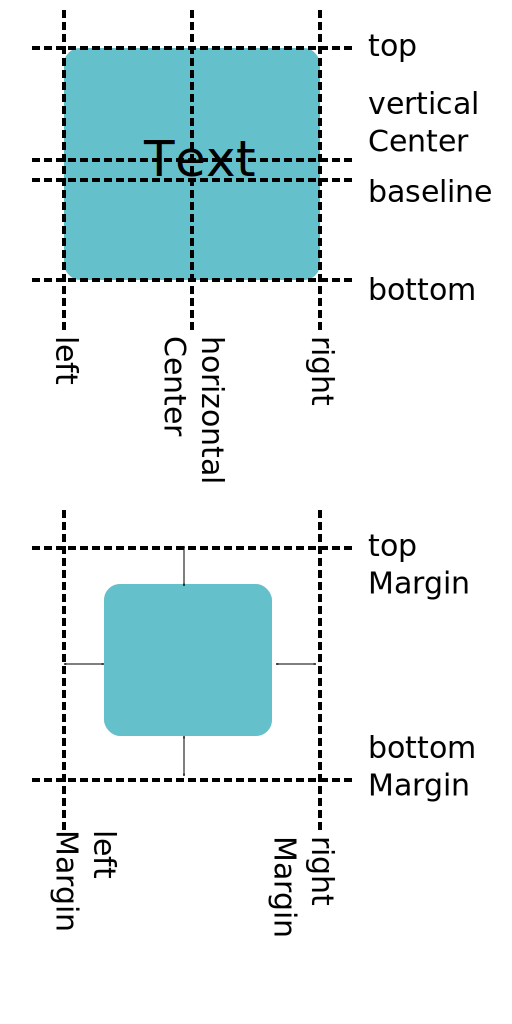
\includegraphics[width=\textwidth]{images/anchors.pdf}
      \end{figure}
    \end{column}
  \end{columns}
\end{frame}

\begin{frame}[fragile]
  \frametitle{Qt Quick -- anchoring examples}
    \footnotesize
    \begin{columns}
      \begin{column}{0.55\textwidth}
      \begin{itemize}
        \item \verb@rect2@ right of \verb@rect1@
        \begin{lstlisting}[basicstyle=\scriptsize\ttfamily]
	Rectangle {
	  id: rect1; ...
	}
	Rectangle {
	  id: rect2; ...
	  anchors.left: rect1.right;
	}
        \end{lstlisting}
        \item \verb@rect2@ bottom right of \verb@rect1@
        \begin{lstlisting}[basicstyle=\scriptsize\ttfamily]
	Rectangle {
	  id: rect1; ...
	}
	Rectangle {
	  id: rect2; ...
	  anchors.left: rect1.right;
	  anchors.top: rect1.bottom;
	}
        \end{lstlisting}
      \end{itemize}
      \end{column}
      \begin{column}{0.45\textwidth}
      \begin{itemize}
        \item \verb@Text@ horizontally centered within its visual parent,
          with fixed vertical position
        \begin{lstlisting}[basicstyle=\tiny\ttfamily]
	Window {
	  width: 320;
	  height: 130;
	  ...

	  Text {
	    text: "My text item"

	    anchors.horizontalCenter:
	      parent.horizontalCenter;
	    y: 40;
	    ...
	  }
	}
        \end{lstlisting}
      \end{itemize}
      \end{column}
    \end{columns}
\end{frame}

\begin{frame}[fragile]
  \frametitle{Qt Quick -- item positioners}
    \footnotesize
    \begin{columns}
      \begin{column}{0.55\textwidth}
      \begin{itemize}
        \item Container items which manage the positions of items in
          a declarative user interface.
        \item Similar to the widget layouts, except that they {\em are} containers.
      \end{itemize}
      \rowcolors{2}{green!80!yellow!50}{green!70!yellow!40}
      \scriptsize
      \begin{tabular}{|p{0.2\textwidth}|p{0.7\textwidth}|}
        \hline
        \textbf{Positioner} & \textbf{Description} \\
        \hline
        Column & Positions children in a column \\
        \hline
        Row & Positions children in a row \\
        \hline
        Flow & Positions children in a row, wrapping as necessary \\
        \hline
        Grid & Positions its children in a grid \\
        \hline
        Layout\-Mirroring & Property used to mirror layout behavior \\
        \hline
      \end{tabular}
      \end{column}
      \begin{column}{0.45\textwidth}
      \begin{itemize}
        \item 
        \begin{lstlisting}[basicstyle=\tiny\ttfamily]
	Item {
	width: 310; height: 170

	  Column {
	    anchors.horizontalCenter:
	      parent.horizontalCenter;
	    anchors.verticalCenter:
	      parent.verticalCenter;

	    spacing: 5

	    Rectangle { ... }
	    Rectangle { ... }
	    Rectangle { ... }

	    Text { ... }
	  }
	}
        \end{lstlisting}
      \end{itemize}
      \end{column}
    \end{columns}
\end{frame}

\begin{frame}
  \frametitle{Qt Quick -- States, Transitions and Animations\footnote
    {\url{doc.qt.io/qt-5.6/qtquick-statesanimations-topic.html}}}
  \small
  \begin{itemize}
    \item Animating between various user interface states can be beneficial
      to the user experience.
    \item Qt Quick provides objects representing the states and changes
      of visual elements:
      \begin{itemize}
        \item States
        \begin{itemize}
          \item Encapsulate particular sets of settings of properties 
          for a visual elements.
          \item Can be hierarchical.
        \end{itemize}
        \item Transitions
        \begin{itemize}
          \item Allow simple smooth transitions between two states, instead
            of abrupt changes.
          \item Use basic interpolation methods.
        \end{itemize}
        \item Behaviors, Animations and Animators
        \begin{itemize}
          \item Allow complex and customizable animations of various item
            properties.
        \end{itemize}
      \end{itemize}
  \end{itemize}
\end{frame}

\begin{frame}
  \frametitle{Qt Quick -- user interaction}
  \begin{itemize}
    \item Depending on the application deployment platform or particular device
      various types of user input can be used in QML applications:
      \begin{itemize}
        \item Mouse -- \texttt{MouseArea}, \texttt{MouseEvent}
        \item Touch-screen -- \texttt{Flickable}, \texttt{MultiPointTouchArea}
        \item Keyboard -- \texttt{Keys}
        \item Device motion sensors -- accelerometer, camera, GPS, thermometers,
          etc., provided by the {\em Qt Sensors}\footnote
          {\url{http://doc.qt.io/qt-5.6/qtsensors-index.html}} module.
      \end{itemize}
      \item Qt signals and slots are used to deliver input interactions.
  \end{itemize}
\end{frame}

\begin{frame}[fragile]
  \frametitle{Qt Quick -- \texttt{MouseArea}\footnote
    {\url{http://doc.qt.io/qt-5.6/qml-qtquick-mousearea.html}}}
  \begin{columns}
    \begin{column}{0.5\textwidth}
    \begin{itemize}
      \item Captures the following mouse interaction events:
      \begin{itemize}
        \small
        \item canceled
        \item clicked
        \item doubleClicked
        \item entered
        \item exited
        \item positionChanged
        \item pressAndHold
        \item pressed
        \item released
      \end{itemize}
    \end{itemize}
    \end{column}
    \begin{column}{0.5\textwidth}
      \begin{lstlisting}[basicstyle=\tiny\ttfamily]
	Window {
	  width: 320; height: 130
	  color: "lightgreen"

	  Text { ... }

	  Text {
	    text: "Close"
	    anchors.bottom:
	      parent.baseline;
	    anchors.horizontalCenter:
	      parent.horizontalCenter;
	    font.pointSize: 12

	    MouseArea {
	      anchors.fill: parent
	      onClicked: Qt.quit()
	    }
	  }
	}
      \end{lstlisting}
    \end{column}
  \end{columns}
\end{frame}

\begin{frame}[fragile]
  \frametitle{Qt Quick -- \texttt{Keys}\footnote
    {\url{http://doc.qt.io/qt-5.6/qml-qtquick-keys.html}}}
  \begin{columns}
    \footnotesize
    \begin{column}{0.55\textwidth}
    \begin{itemize}
      \item Implements key press handling functionality
      \item Visual items have the \texttt{Keys} attached property to enable
        key events.
      \item Keyboard events are generally handled in two signal properties:
      \begin{itemize}
        \scriptsize
        \item pressed
        \item released
      \end{itemize}
      \item Special keys have their own signal handlers:
      \begin{itemize}
        \scriptsize
        \item noPressed
        \item yesPressed
        \item upPressed
        \item downPressed
        \item leftPressed
        \item rightPressed
        \item \ldots
      \end{itemize}
    \end{itemize}
    \end{column}
    \begin{column}{0.45\textwidth}
      \begin{lstlisting}[basicstyle=\tiny\ttfamily]
	Rectangle {
	  anchors.fill: parent
	  focus: true

	  Keys.onUpPressed: {
	    console.log("move up");
	    event.accepted = true;
	  }

	  Keys.onDownPressed: {
	    console.log("move down");
	    event.accepted = true;
	  }

	  Keys.onPressed: {

	    if (event.key == Qt.Key_Left) {

	      console.log("move left");
	      event.accepted = true;
	    }
	    if (event.key == Qt.Key_Right) {

	      console.log("move right");
	      event.accepted = true;
	    }
	  }
	}
      \end{lstlisting}
    \end{column}
  \end{columns}
\end{frame}

\begin{frame}
  \frametitle{Qt Quick -- controls\footnote
    {\url{http://doc.qt.io/qt-5.6/qtquickcontrols-index.html}} -- Main window}
  \rowcolors{2}{green!80!yellow!50}{green!70!yellow!40}
  \begin{tabular}{|p{0.3\textwidth}|p{0.6\textwidth}|}
        \hline
        \textbf{Control} & \textbf{Description} \\
        \hline
        Action & Abstract user interface action that can be bound to items \\
        \hline
        ApplicationWindow & Provides a top-level application window \\
        \hline
        MenuBar & Provides a horizontal menu bar \\
        \hline
        StatusBar & Contains status information in your app \\
        \hline
        ToolBar & Contains ToolButton and related controls \\
        \hline
  \end{tabular}
\end{frame}

\begin{frame}
  \frametitle{Qt Quick -- controls\footnote
    {\url{http://doc.qt.io/qt-5.6/qtquickcontrols-index.html}} -- Navigation and views}
  \rowcolors{2}{green!80!yellow!50}{green!70!yellow!40}
  \begin{tabular}{|p{0.2\textwidth}|p{0.7\textwidth}|}
        \hline
        \textbf{Control} & \textbf{Description} \\
        \hline
        ScrollView & Provides a scrolling view within another Item \\
        \hline
        SplitView & Lays out items with a draggable splitter between each item \\
        \hline
        StackView & Provides a stack-based navigation model \\
        \hline
        TabView & A control that allows the user to select one of multiple stacked items \\
        \hline
        TableView & Provides a list view with scroll bars, styling and header sections \\
        \hline
        TreeView & Provides a tree view with scroll bars, styling and header sections \\
        \hline
  \end{tabular}
\end{frame}

\begin{frame}
  \frametitle{Qt Quick -- controls\footnote
    {\url{http://doc.qt.io/qt-5.6/qtquickcontrols-index.html}} -- Common}
  \rowcolors{2}{green!80!yellow!50}{green!70!yellow!40}
  \footnotesize
  \begin{tabular}{|p{0.2\textwidth}|p{0.7\textwidth}|}
        \hline
        \textbf{Control} & \textbf{Description} \\
        \hline
        Button & A push button with a text label \\
        \hline
        CheckBox & A checkbox with a text label \\
        \hline
        ComboBox & Provides a drop-down list functionality \\
        \hline
        GroupBox & Group box frame with a title \\
        \hline
        Label & A text label \\
        \hline
        Menu & Provides a menu component for use as a context menu, popup menu,
          or as part of a menu bar \\
        \hline
        ProgressBar & A progress indicator \\
        \hline
        Slider & Provides a vertical or horizontal slider control \\
        \hline
        SpinBox & Provides a spin box control \\
        \hline
        StatusBar & Contains status information in your app \\
        \hline
        Switch & A switch \\
        \hline
	TextArea & Displays multiple lines of editable formatted text \\
        \hline
	TextField & Displays a single line of editable plain text \\
        \hline
	ToolBar & Contains ToolButton and related controls \\
        \hline
  \end{tabular}
\end{frame}

 \begin{frame}[fragile]
  \frametitle{Qt QML\footnote{\url{http://doc.qt.io/qt-5.6/qtqml-index.html}}}
  \small
  \begin{itemize}
    \item Defines and implements the QML language and engine infrastructure.
    \item Implements commonly used QML types.
    \item Framework for developing applications and libraries using the QML
      language. 
    \item Framework for running JavaScript expressions in QML and from C++.
    \item Using from C++
    \begin{itemize}
      \item \verb@#include <QtQml>@
    \end{itemize}
    \item Using from QML
    \begin{itemize}
      \item \verb@import QtQml 2.0@
    \end{itemize}
    \item Project files
    \begin{itemize}
      \item \verb@QT += qml@
    \end{itemize}
  \end{itemize}
\end{frame}

 \begin{frame}[fragile]
  \frametitle{Integration with C++ -- simple Qt Quick application}
  \begin{lstlisting}
	#include <QtCore>
	#include <QGuiApplication>
	#include <QQuickView>
	#include <QUrl>

	int main(int argc, char** argv)
	{
	    QGuiApplication app(argc, argv);
	    QQuickView qmlview(QUrl("qrc:///semaphore.qml"));
	    qmlview.show();
	    return app.exec();
	}
  \end{lstlisting}
\end{frame}

 \begin{frame}[fragile]
  \frametitle{Integration with C++ -- QML resources}
  \begin{lstlisting}
	<!DOCTYPE RCC><RCC version="1.0">
	<qresource>
	    <file>SemLight.qml</file>
	    <file>semaphore.qml</file>
	    <file>stop.svg</file>
	    <file>walk.svg</file>
	</qresource>
	</RCC>
  \end{lstlisting}
\end{frame}

 \begin{frame}[fragile]
  \frametitle{Integration with C++ -- Implementing QML object}
  \begin{lstlisting}[basicstyle=\scriptsize\ttfamily]
	class SemManager
 	 : public QObject
	{
	    Q_OBJECT
	    Q_PROPERTY(QString semState
	               READ getSemState
	               NOTIFY semStateChanged
	    )

	    bool _stop;
	public:
	    SemManager(QObject* parent = 0);

	    QString getSemState(void) const;
	signals:
	    void semStateChanged(void);
	public slots:
	    void activate(void);
	    void stop(void);
	    void go(void);
	};
  \end{lstlisting}
\end{frame}

 \begin{frame}[fragile]
  \frametitle{Integration with C++ -- Using custom QML object}
  \begin{itemize}
  \item Registering in C++
  \begin{lstlisting}[basicstyle=\scriptsize\ttfamily]
	qmlRegisterType<SemManager>(
	    "sk.uniza.fri.qt",
	    1, 0,
	    "SemManager"
	);
  \end{lstlisting}
  \item Importing in QML
  \begin{lstlisting}[basicstyle=\scriptsize\ttfamily]
	import sk.uniza.fri.qt 1.0
  \end{lstlisting}
  \item Using in QML
  \begin{lstlisting}[basicstyle=\scriptsize\ttfamily]
	SemManager { id: "manager" }

	MouseArea {
	    anchors.fill: parent
	    onClicked: manager.activate()
	}
  \end{lstlisting}
  \end{itemize}
\end{frame}

 \begin{frame}[fragile]
  \frametitle{Integration with C++ -- Qt Quick controls application}
  \begin{lstlisting}[basicstyle=\scriptsize\ttfamily]
	#include <QtCore>
	#include <QGuiApplication>
	#include <QQmlApplicationEngine>
	#include <QQuickView>
	#include <QtQml>
	#include <QUrl>

	int main(int argc, char** argv)
	{
	    QGuiApplication app(argc, argv);

	    QQmlApplicationEngine engine;
	    engine.load(QUrl("qrc:///main.qml"));

	    QObject* root = engine.rootObjects().value(0);
	    QQuickWindow* win = qobject_cast<QQuickWindow*>(root);
	    win->show();

	    return app.exec();
	}
  \end{lstlisting}
\end{frame}



% Internationalization % 
\section{Localization}
\subsection{Translations and internationalization}

\begin{frame}
  \frametitle{Localization overview\footnote
    {\url{https://wiki.qt.io/QtInternationalization}}}
  \begin{itemize}
    \item Translation of user interface texts to user language
    \begin{itemize}
      \item Left-to-right, right-to-left scripts.
      \item Plural forms.
    \end{itemize}
    \item Displaying information in region-specific format.
    \begin{itemize}
      \item date and time,
      \item numbers and currency,
      \item \ldots
    \end{itemize}
    \item Other considerations
    \begin{itemize}
      \item time-zones,
      \item color sensitivities,
      \item cultural references and habits,
      \item \ldots
    \end{itemize}
  \end{itemize}
\end{frame}

\begin{frame}
  \frametitle{Basic workflow}
  \small
  \begin{itemize}
    \item Mark all text literals which are to be translated in the source.
    \item Update the project files.
    \item Invoke the \texttt{lupdate} tool to generate the \texttt{.ts} files.
    \item Update the \texttt{.ts} translation XML files -- translate the texts
      into a particular language.
    \item Invoke the \texttt{lrelease} tool to generate the \texttt{.qm} binary
      translation files.
    \item Update the application source to load and apply the translations.
    \item Use the \texttt{QLocale} class to convert between numbers and strings
      in locale-specific formats.
  \end{itemize}
\end{frame}

\begin{frame}[fragile]
  \frametitle{Marking texts in source}
  \begin{itemize}
    \item All text literals which should be translated into user's language
     should be wrapped in the \texttt{tr()}\footnote{in C++} or the
      \texttt{qsTr()}\footnote{in QML} macros.
    \item Basic variant
    \begin{itemize}
      \item \verb@tr("&Application")@
      \item \verb@qsTr("&File")@
    \end{itemize}
    \item Disambiguation
    \begin{itemize}
      \item \verb@tr("&Open", "file")@
      \item \verb@tr("&Open", "window")@
      \item \verb@tr("&Open", "network connection")@
    \end{itemize}
    \item Plurals
    \begin{itemize}
      \item \verb@tr("%1 items(s) loaded", "", n)@
      \item \verb@tr("%1 file(s) remaining", "progress", n)@
    \end{itemize}
  \end{itemize}
\end{frame}

\begin{frame}[fragile]
  \frametitle{Updating project files}
  \begin{itemize}
    \item The \texttt{TRANSLATIONS} variable in the project files should
     be updated to contain the names of the translation XML files.
     \begin{lstlisting}
	TRANSLATIONS += myapp_sk.ts
	TRANSLATIONS += myapp_de.ts
	TRANSLATIONS += myapp_fr.ts
     \end{lstlisting}
    \item The \texttt{SOURCES} variable determines which source files should
     be scanned.
    \item It is possible to add sources only for the \texttt{lupdate} tool:
     \begin{lstlisting}
	lupdate_only {
	    SOURCES += gui.qml
	    SOURCES += helper.qml
	}
     \end{lstlisting}
  \end{itemize}
\end{frame}

\begin{frame}[fragile]
  \frametitle{\texttt{lupdate}\footnote
   {\url{http://doc.qt.io/qt-5.6/linguist-manager.html\#lupdate}}}
  \begin{itemize}
    \item The \texttt{lupdate} tool scans the source files and searches for
      marked string literals.
    \item Generates the \texttt{.ts}, XML-based translation files.
    \item Basic usage
    \begin{itemize}
      \item \verb@lupdate project.pro@
      \item \verb@lupdate src.cpp src.qml ... -ts output.ts@
    \end{itemize}
  \end{itemize}
\end{frame}

\begin{frame}[fragile]
  \frametitle{Translating the \texttt{.ts} files}
  \small
  \begin{itemize}
    \item The generated \texttt{.ts} files contain the original strings extracted
      from the source files.
    \item Each \texttt{.ts} file contains the translation of the interface
      to a single language.
    \item These files should be translated by the translators to the target
      language.
  \end{itemize}
  \begin{lstlisting}[basicstyle=\tiny\ttfamily]
<!DOCTYPE TS>
<TS version="2.1">
<context>
    <name>primes</name>
    <message>
        <location filename="primes.qml" line="16"/>
        <source>Quit</source>
        <comment>application</comment>
        <translation>Ukoncit</translation>
    </message>
    <message>
        <location filename="primes.qml" line="23"/>
        <source>Start</source>
        <translation>Spustit</translation>
    </message>
</context>
</TS>
  \end{lstlisting}
\end{frame}

\begin{frame}[fragile]
  \frametitle{\texttt{lrelease}\footnote
   {\url{http://doc.qt.io/qt-5.6/linguist-manager.html\#lrelease}}}
  \begin{itemize}
    \item The \texttt{lrelease} tool converts the XML-based \texttt{.ts} files
      into a more efficient binary representation which is loaded by the
      application.
    \item Basic usage
    \begin{itemize}
      \item \verb@lrelease project.pro@
      \item \verb@lrelease file_sk.ts  ... -qm output.qm@
    \end{itemize}
  \end{itemize}
\end{frame}

\begin{frame}[fragile]
  \frametitle{Loading translation in a QML/C++ application}
  \small
  \begin{itemize}
   \item The binary translation files can be embedded as resources:
   \begin{lstlisting}[basicstyle=\scriptsize\ttfamily]
	<!DOCTYPE RCC><RCC version="1.0">
	<qresource>
	    <file>primes.qml</file>
	    <file>primes_sk.qm</file>
	</qresource>
	</RCC>
   \end{lstlisting}
   \item The \texttt{QTranslator}\footnote
     {\url{http://doc.qt.io/qt-5.6/qtranslator.html}} class can be used to load
     a translation and register it with the application
   \begin{lstlisting}[basicstyle=\scriptsize\ttfamily]
	QGuiApplication app(argc, argv);

	QTranslator translator;
	if(translator.load(":/primes_sk.qm")) {
	    app.installTranslator(&translator);
	}
   \end{lstlisting}
  \end{itemize}
\end{frame}

\begin{frame}[fragile]
  \frametitle{\texttt{QLocale}\footnote
   {\url{http://doc.qt.io/qt-5.6/qlocale.html}}}
  \begin{itemize}
    \item Converts data like numbers, date and time, currency, etc. between
      their numeric value and string representation in a specified language.
   \item Enumerations
   \begin{itemize}
     \small
     \item \texttt{QLocale::Language}
     \item \texttt{QLocale::Script}
     \item \texttt{QLocale::Country}
     \item \texttt{QLocale::MeasurementSystem}
     \item \ldots
   \end{itemize}
   \item Construction:
   \begin{itemize}
     \small
     \item \verb@QLocale::system()@ -- system locale
     \item \verb@QLocale(const QString& name)@ -- \verb@sk_SK@, \verb@en_US@,
       \verb@de_DE@, etc.
     \item \verb@QLocale(Language, Country)@
     \item \verb@QLocale(Language, Script, Country)@
   \end{itemize}
  \end{itemize}
\end{frame}

\begin{frame}
  \frametitle{\texttt{QLocale} -- functions}
  \small
  \begin{itemize}
    \item \texttt{country}, \texttt{language}, \texttt{script}, \texttt{name}
    \item \texttt{nativeCountryName}, \texttt{nativeLanguageName}
    \item \texttt{textDirection},
    \item \texttt{dateFormat}, \texttt{timeFormat}, \texttt{dateTimeFormat}
    \item \texttt{currencySymbol}, \texttt{percent}, \texttt{zeroDigit},
      \texttt{exponential}
    \item \texttt{positiveSign}, \texttt{negativeSign}, \texttt{decimalPoint},
      \texttt{groupSeparator}
    \item \texttt{toString}, \texttt{toCurrencyString}
    \item \texttt{toInt}, \texttt{toFloat}, \texttt{toDouble},
      \texttt{toDate}, \texttt{toTime}, etc.
    \item \texttt{toUpper}, \texttt{toLower}
      
  \end{itemize}
\end{frame}



 \begin{frame}[fragile]
  \frametitle{QML examples}
  \small
  \begin{itemize}
    \item Located in the \verb@examples\03_qml\@ directory
    \begin{itemize}
      \item \verb@01_sem_basic@ -- simple two-light semaphore controlled by two
        \say{buttons}. Shows the concept and usage of states.
      \item \verb@02_sem_basic@ -- extends the previous example with state
        transitions.
      \item \verb@03_sem_timer@ -- extends the previous example with Timers and
        Images.
      \item \verb@04_sem_cpp@ -- shows how to implement the semaphore-controlling
        logic in C++ instead of directly in QML. Also shows how to implement
        custom visual items in QML.
      \item \verb@05_primes@ -- simple calculator of prime numbers. Shows the
        Qt Quick controls library, Qt Quick actions and layouts. Implements
        the logic in C++.
      \item \verb@06_translation@ -- adds UI text translation to the previous
        example.
      \item \verb@07_plurals@ -- shows how to handle number plural forms in
        localized texts.
    \end{itemize}
  \end{itemize}
\end{frame}



% Outro %
\section{Conclusion}

\subsection{Thank you}
\begin{frame}
\begin{center}
\Huge{Thank you!}
\end{center}
\end{frame}



\end{document}
